\part{Soluções Apresentadas}
\label{sol}
\chapter[Estruturas e Materiais]{Estruturas e Materiais}

\section{Otimização da Planta}
\subsection{Adaptações da planta}
As soluções apresentadas para a parte estrutural do projeto são apenas sugestões, visto que as decisões efetivas devem ser feitas por um profissional de engenharia civil, de soluções para os problemas que o prédio UAC (Unidade Acadêmica) apresenta, cuja a planta baixa foi usada para a análise dos problemas, visando uma estrutura que aproveite melhor os recursos naturais e seja mais sustentável.
Similarmente, para realizar este projeto, foi necessária uma adaptação de elementos relativos a automação predial à um projeto de construção civil comum com integração do sistema Smart Grid, dando ênfase na sustentabilidade. Também foi necessária a integração entre de uma sala de controle para o sistema de automação do prédio.
Um sistema de automação pode ser centralizado ou distribuído. Os centralizados são aqueles que utilizam uma seção especificamente para o controle dos dispositivos, tanto para receber quanto enviar sinais. Os sistemas distribuídos são considerados descentralizados porque utilizam de diversos dispositivos, cada um com uma função específica dentro do sistema, sendo distribuídos por toda instalação e interligados por uma rede (Dias, 2004).
Considerando que a rede de automação a ser implementada possui um sistema centralizado, viu-se a necessidade de um local específico para controlar e monitorar o sistema. Já para promover a integração do Smart Grid ao projeto, foi constatado que o melhor ponto para a instalação das placas fotovoltaicas seria no telhado, onde há maior contato com sol, menor projeção de sombras e resguardado de contato de animais e pessoas. Quanto à posição da placa, esta deverá estar voltada para o norte.
A função das salas foi baseada na necessidade do prédio, a qual consta adicionar mais salas de aula e de laboratório no campus. Dada a quantidade de alunos que ingressam todo semestre, somente os prédios atuais não são capazes de atender a demanda, são providas cerca de 140 vagas pelo Vestibular da Universidade de Brasília e pelo ENEM, com a pouca quantidade de formaturas por semestre, o campus está sobrecarregado.
Considerando a efetiva carência foi estabelecido que as salas do pavimento inferior serão designadas para laboratórios, enquanto as do pavimento superior cumprirão função de salas de aulas. Haverá adicionalmente uma sala de estudos no lugar que se dispõe a biblioteca do prédio atual de salas e no lugar da secretaria, no prédio inteligente constará a sala de controle. O pavimento superior também contará com um espaço para Xerox e ao lado, mais salas.

\begin{figure}[!ht]
  \centering
  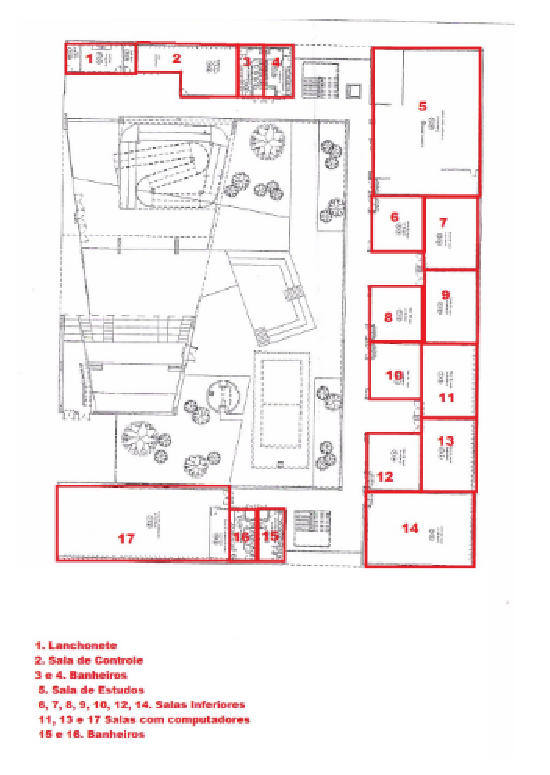
\includegraphics[keepaspectratio=true,scale=1]{figuras/plantabaixa1.eps}
  \caption{Planta Baixa com finalidade das salas - Piso Inferior}
  \label{fig:planta_salas_inferior}
\end{figure}

\begin{figure}[!ht]
  \centering
  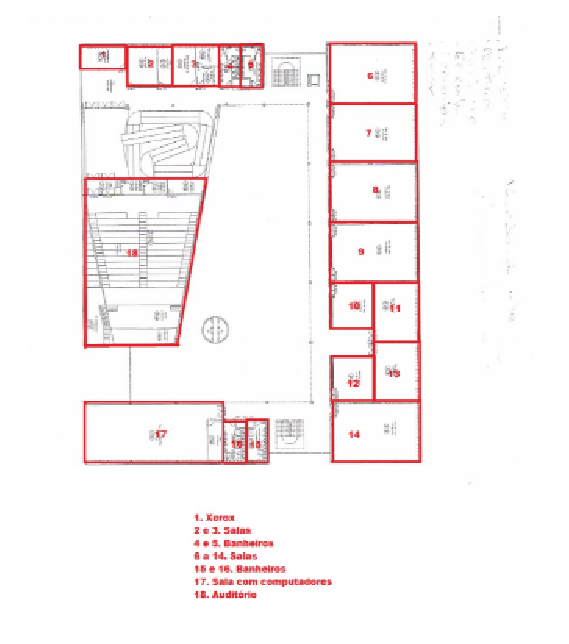
\includegraphics[keepaspectratio=true,scale=1]{figuras/plantabaixa2.eps}
  \caption{Planta baixa com finalidade das salas - Piso superior}
  \label{fig:planta_salas_superior}
\end{figure}

O motivo para a realização da modelagem 3D do prédio é a facilidade de ver como será o prédio após a sua construção.Além de facilitar a visualização de qualquer problema que tenha passado despercebido na planta. Também facilita prever como as pessoas passarão pelo prédio e como também elas poderão se acomodar dentro do mesmo. Um desenho em duas dimensões não é capaz de passar a quantidade de informações que um modelo em três dimensões passa para seu observador.

\begin{figure}[!ht]
  \centering
  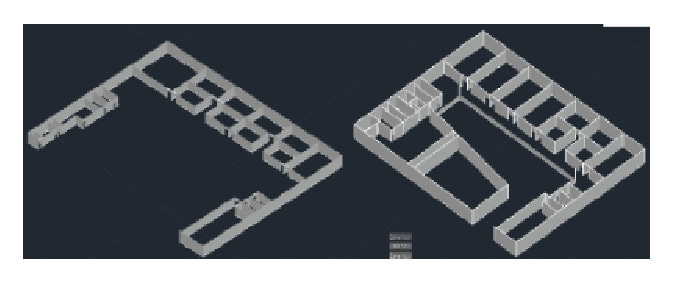
\includegraphics[keepaspectratio=true,scale=1]{figuras/modelagemautocad.eps}
  \caption{Modelagem 3D- Pisos inferior e superior da esquerda para direita}
  \label{fig:modelagem_3d}
\end{figure}

\section{Poeira e Climatização}

Um dos problemas mais latentes observado pelos usuários do prédio é a temperatura elevada que permanece nas salas, o que causa grande desconforto para os mesmo. Para encontrar uma solução, foi analisado a relação da incidência solar com posicionamento do prédio. Dessa forma, por meio do programa SOL-AR 6.2 fornecido pela UFSC, foi possível obter a carta solar de Brasília para análise do melhor posicionamento do novo prédio do campus da FGA.

\begin{figure}[!ht]
  \centering
  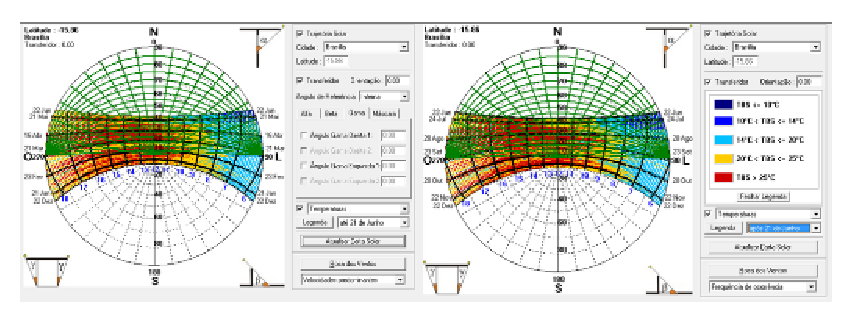
\includegraphics[keepaspectratio=true,scale=1]{figuras/cartasolar.eps}
  \caption{Carta Solar de Brasília: até junho e após junho respectivamente}
  \label{fig:carta_solar}
\end{figure}

O resultado da carta solar é um par de eixos ordenado com o eixo das abcissas representando a hora do dia variando de 6 às 18 e o eixo das ordenadas representa os dias do ano e cada ponta desse par de eixos representa uma direção geográfica (Norte, Sul, Leste e Oeste) e a partir do sistema de cores é possível fazer o estudo da região. Analisando os resultados obtidos nota-se que o Leste apresenta uma radiação mais amena do que a Oeste que conta com grande irradiação solar, ou seja, maior temperatura ao longo do dia. Como as salas de aula são lugares de longa permanência o ideal é que elas fiquem voltadas ao Leste devido a temperatura se manter mais amena ao longo do dia.

\begin{figure}[!ht]
  \centering
  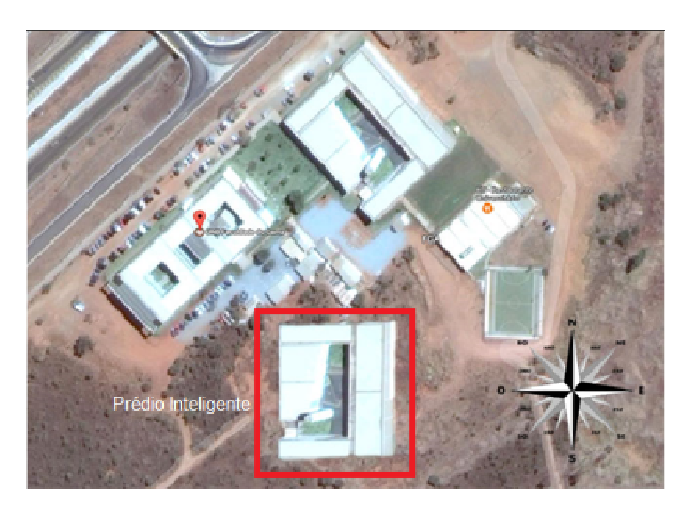
\includegraphics[keepaspectratio=true,scale=1]{figuras/posicionamentodoprediointeligente.eps}
  \caption{Posicionamento do Prédio Inteligente}
  \label{fig:posicionamento}
\end{figure}

Porém como o Sol nasce ao leste seu reflexo poderia atrapalhar o rendimento das aulas. Problema esse que pode ser resolvido com o bom posicionamento de brises para diminuir a incidência solar dentro da sala de aula. Essas estruturas já existem no prédio atual, mas poderiam ser substituídos pelo brise que acompanha o trajeto solar.
Outro problema que aflige a estrutura é a poeira proveniente dos arredores do campus, problema este que também pode ser amenizado com os brises mencionados anteriormente e também com uso de cobogós e jardins verticais. Porém, com exceção do jardim vertical, os brises e cobogós já foram implementados no prédio atual. Dessa forma, cabe fazer a análise de jardins verticais como recurso para amenizar o problema.
O ar do Gama é muito seco o que favorece a permanência da poeira no ar, além de secar as vias respiratórias. Dessa forma o controle da umidade é essencial para mitigar o problema da poeira no campus. Algumas soluções podem ser tomadas para aumentar a umidade ar como a arborização no campus e uso de jardins verticais. Estas foram escolhidas para o projeto pois apresentam certas vantagens como descrito na tabela. A água para irrigação das árvores e dos jardins poderá ser proveniente do poço já existente que abastece o campus ou também por um reservatório que reaproveita água da chuva. Para o último, o dimensionamento dependerá de diversos fatores que vão além do escopo deste projeto como: tipo de irrigação e vazão do mecanismo, espécie de planta a ser usada e litros/dia de água que esses recursos vão necessitar, além da análise de temporadas de chuvas na região do DF.

\begin{figure}[!ht]
  \centering
  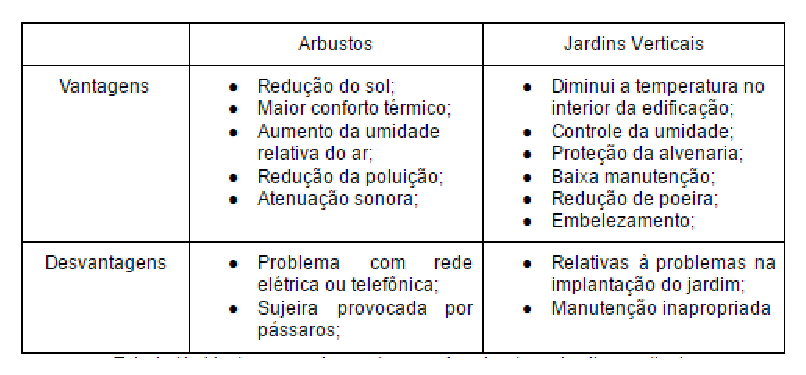
\includegraphics[keepaspectratio=true,scale=1]{figuras/tabela_vantagens_e_desvantagens_do_jardim_vertical.eps}
  \caption{Tabela com vantagens e desvantagens de arbustos e jardins verticais}
  \label{fig:comparativo_jartins}
\end{figure}

Além desse recurso natural, faz-se necessário o uso de um climatizador para solucionar o desconforto provocado pela poeira, que impede um uso mais eficaz das janelas. Segue uma tabela comparativa do recursos considerados para a solução.

\begin{figure}[!ht]
  \centering
  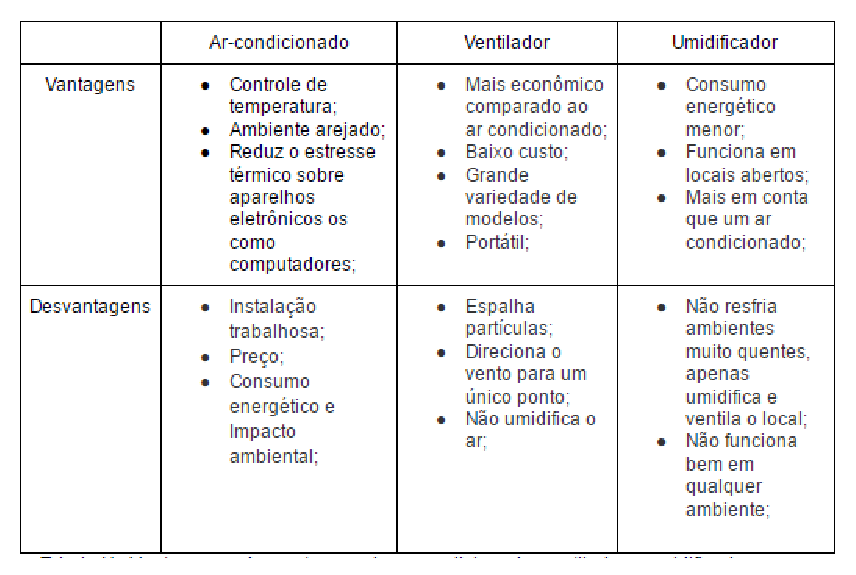
\includegraphics[keepaspectratio=true,scale=1]{figuras/tabela_vantagens_e_desvantagens_do_climatizador.eps}
  \caption{Tabela com vantagens e desvantagens do uso de ar-condicionados,climatizadores e ventiladores}
  \label{fig:comparativo_climatizador}
\end{figure}

No entanto, para que se possa saber qual o tipo de climatizador ideal para a sala de aula, deve-se primeiramente calcular a carga térmica do ambiente a ser climatizado, e isso é uma tarefa complicada, pois necessita de uma gama de variáveis, tais como área e volume do local, número de pessoas que irão ocupar a sala de aula, número de aparelhos que emitem calor(tal como computadores e aparelhos de TV) , posicionamento geográfico das paredes em relação ao sol, bem como a quantidade de janelas presentes na sala de aula.
Então para facilitar, utilizou-se de um software que calcula a carga térmica (disponível no site de um fabricante).Para fins de padronização, utilizou-se das medidas das maiores salas de aula da FGA, pois são as que apresentam o maior valor de carga térmica, visto que, os climatizadores devem atender a demanda de todas as salas, e para tal, deve-se escolher ar-condicionados que suportem pelo menos a maior carga térmica presente.

\begin{figure}[!ht]
  \centering
  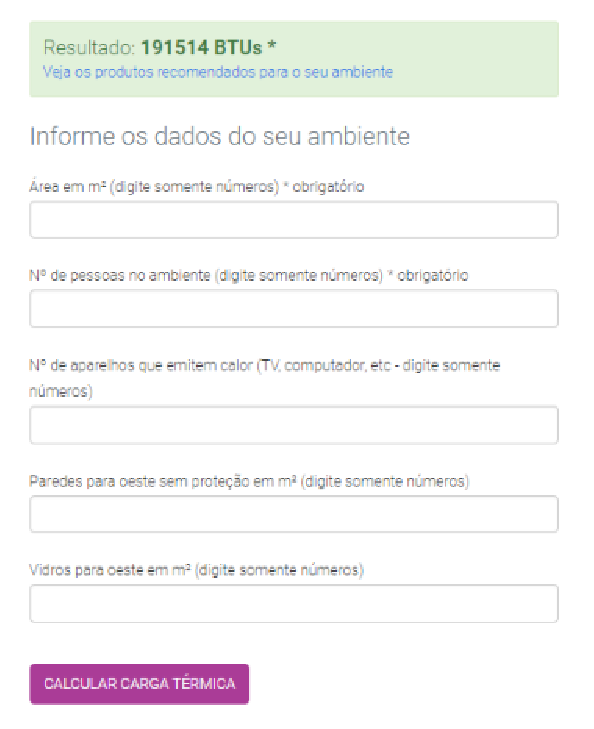
\includegraphics[keepaspectratio=true,scale=1]{figuras/interface_calculo_carga_termica.eps}
  \caption{Interface do software que calcula a carga térmica}
  \label{fig:calculo_carga_termica}
\end{figure}

Para fins de cálculo, as variáveis utilizadas para calcular a carga térmica foram as seguintes:
\\
Área: (9.555x13.63)$m^2$
\\
Número de pessoas no ambiente quando a sala está cheia: 120 pessoas
\\
Número de aparelhos que emitem calor: 30 aparelhos ( incluindo datashow e laptops)
\\
Paredes na direção oeste em $m^2$: (9.555x3.5)$m^2$
Vidros para o oeste em $m^2$: 16.72$m^2$
\\
Ao utilizar o software, estimou-se que a carga térmica média de uma sala de aula grande com base nos dados anteriores é em média 191514 BTU
Para suprir a demanda, terá que ser utilizado pelo menos 3 ar condicionados do tipo
Komeco Piso Teto V, 22.000 à 60.000 BTU/h frio, que custa em média 6200 reais em lojas de climatizadores

\begin{figure}[!ht]
  \centering
  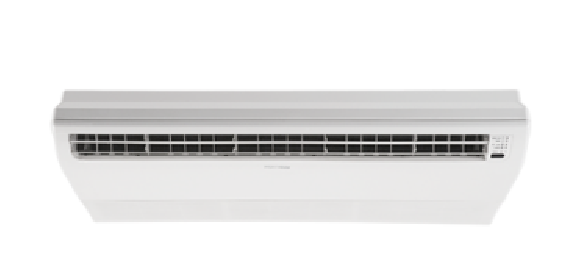
\includegraphics[keepaspectratio=true,scale=1]{figuras/arcondicionado.eps}
  \caption{Climatizador do tipo Komeco Piso Teto V, 22.000 à 60.000 BTU/h frio}
  \label{fig:climatizador}
\end{figure}

Já para as salas menores serão consideradas as seguintes dimensões para o cálculo da carga térmica:
\\
-Área :(11.27x8)$m^2$
\\
-Número de pessoas no ambiente: 60 pessoas
\\
-Número de aparelhos que emitem calor:50 (no caso das salas com computadores I6 e I7)
\\
-Paredes para o oeste em $m^2$ : (11.27x2.71)$m^2$
\\
-Vidros para o oeste : 7.63$m^2$
\\
Ao utilizar por os dados acima no software, estimou-se que a carga térmica das menores salas é em média 120000 BTUs, o que convém instalar em cada sala 2 climatizadores do tipo Komeco Piso Teto V, 22.000 à 60.000 BTU/h frio. Estimativa de custos:

\section{Viabilidade das soluções}
\subsection{Brises}
Para a instalação dos brises (quebra Sol) estima-se um valor de R\$ 789,64 reais por metro quadrado ($m^2$). Dessa forma, utilizando a planta e estimando uma altura pouco maior que a janela ocupa e usando a largura da face do prédio que possui mais janelas da sala, obtém-se R\$362.965,92 de custo.

\begin{figure}[!ht]
  \centering
  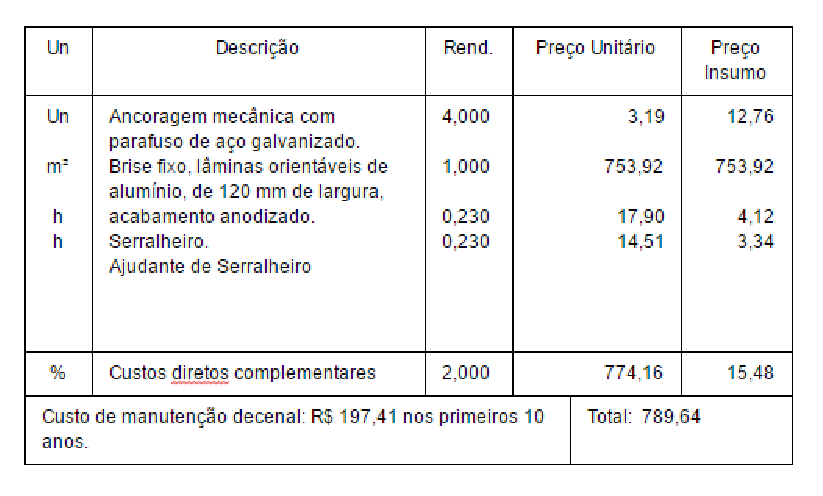
\includegraphics[keepaspectratio=true,scale=1]{figuras/tabelapreco.eps}
  \caption{Preço de instalação para o brise}
  \label{fig:preco_brise}
\end{figure}

\begin{figure}[!ht]
  \centering
  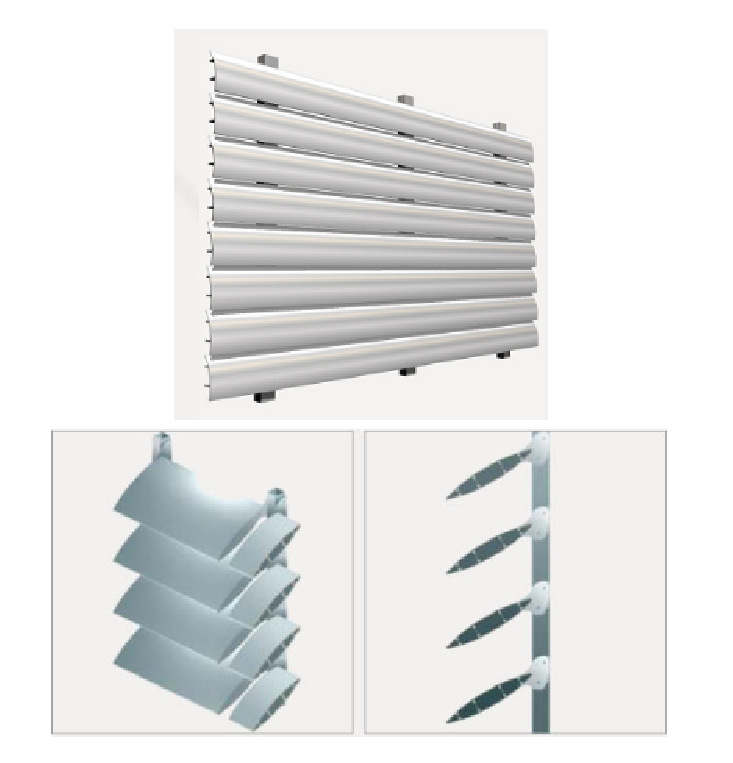
\includegraphics[keepaspectratio=true,scale=1]{figuras/brises.eps}
  \caption{Brises}
  \label{fig:brises}
\end{figure}

Apesar dos brises apresentarem um valor alto deve-se levar em consideração que eles podem proporcionar redução no consumo de energia e trazer bem-estar as pessoas, além disso os brises de alumínio apresentam outras vantagens tais como: redução da carga térmica, desempenho térmico e luminoso, permite ventilação e visibilidade, pode ser adaptável a diversos tipos de obras, excelente vida útil, alta resistência a impactos, 100\% reciclável, potencial termoacústico e o alumínio não apresenta toxicidade.  “A previsão de custo considera apenas a execução de obra. Não é avaliada a relação custo-benefício obtido com a economia da eficiência térmica do dispositivo, com a redução do consumo de energia para condicionamento artificial. Em relação a ambientes de trabalho e estudo, pesquisas mostram que o conforto do usuário tem impacto direto na produtividade do trabalhador e aprendizagem de alunos” – Grace Gutierrez, arquiteta urbanista e mestre em Engenharia Civil pela Unicamp. 

\section{Jardins verticais}
Como previsto, a utilização de jardins verticais além de dar enfoque à questão da sustentabilidade, ameniza o dispêndio de energia, proporciona melhoria na qualidade do ar no interior e nos arredores do edifício, beneficia a acústica do ambiente e é esteticamente vantajoso. Dentre as opções de jardins verticais, tem-se a de fachada verde e a de parede verde:

\begin{figure}[!ht]
  \centering
  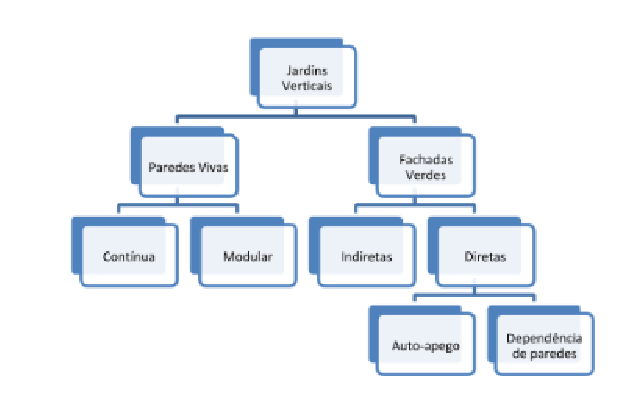
\includegraphics[keepaspectratio=true,scale=1]{figuras/jardimvertical.eps}
  \caption{Tipos de jardins verticais}
  \label{fig:tipos_jardins_verticais}
\end{figure}

Para avaliação relativa às técnicas, foi utilizado um quadro comparativo entre as opções levantadas para a instalação: 

\begin{figure}[!ht]
  \centering
  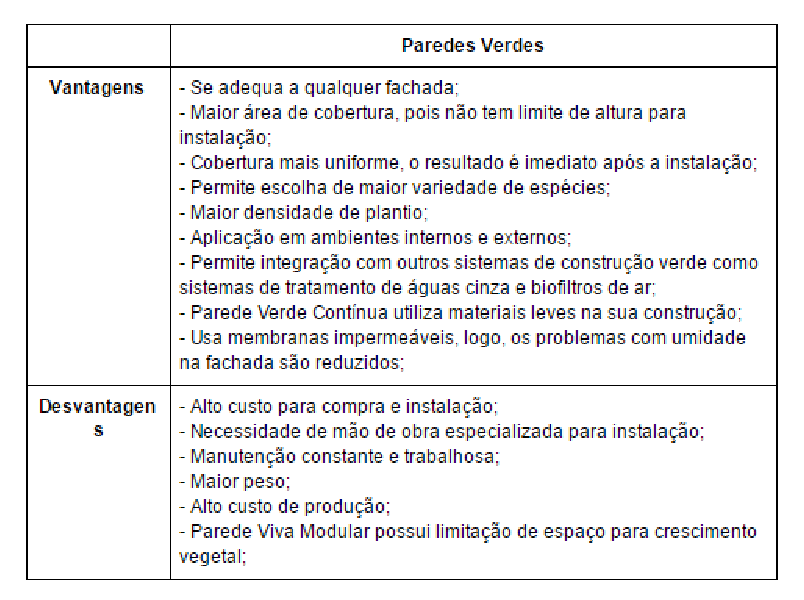
\includegraphics[keepaspectratio=true,scale=1]{figuras/comparativo_de_paredes_verdes.eps}
  \caption{Comparativo de paredes verdes}
  \label{fig:comparativo_paredes_verdes}
\end{figure}

\begin{figure}[!ht]
\centering
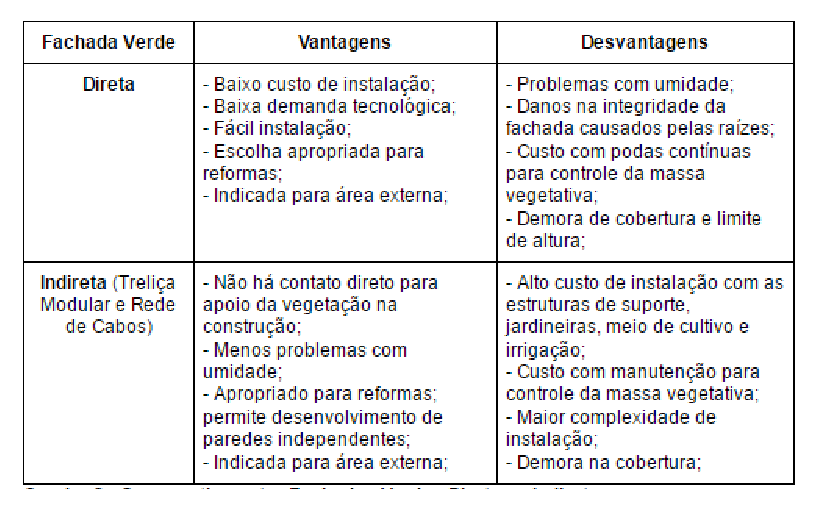
\includegraphics[keepaspectratio=true,scale=1]{figuras/comparativo_de_fachadas_verdes_diretas_e_indiretas.eps}
\caption{Comparativo de fachadas verdes diretas e indiretas}
\end{figure}

Para a definição da técnica utilizada foram utilizados os seguintes requisitos: ter uma estrutura que seja apropriada para altura do prédio, seja indicada para área externa, cumpra com os propósitos iniciais de sua instalação, utilize um método de irrigação que faça reutilização de água e/ou tenha baixa exigência hídrica, seja economicamente viável e não comprometa a estrutura do prédio.
A escolha das plantas deve ser de acordo com a incidência de sol, vento e chuva, e de preferência que não necessitem de muitos recursos hídricos e nutricionais. Para reduzir o gasto com manutenção, serão utilizadas plantas perenes, que possuem um ciclo de vida mais longo e plantas epífitas ou rupícolas, que são plantas que se apoiam sobre outras plantas sem retirar seus nutrientes ou plantas que vivem apoiadas sobre muros e paredes.
Por mais que a escolha da parede viva tenha diversas vantagens, como maior e mais rápida cobertura, variedade de plantas, sua viabilidade econômica é muito baixa. Utilizando orçamentos colhidos com as empresas “ALS Jardins, Paisagismo e Irrigação” e “Vertical Paisagismo”, a despesa da instalação já com os materiais e sistema de irrigação custa por volta de R\$1200 o $m^2$. Já a utilização da fachada verde indireta, com auxílio de treliças e cabos de aço e com o uso de trepadeiras, custa por volta de R\$700 o $m^2$, com materiais e sistema de irrigação. Esta, por sua vez, apesar de possuir uma cobertura em longo prazo, não impõe riscos à estrutura e para reduzir o custo com a manutenção, podem ser usados dois tipos de trepadeira, a “unha de gato” ou a “hera”. Seu sistema de irrigação é automatizado e controlado para reduzir o gasto de água e pode ser integrado ao sistema de captação de água da chuva. Sua instalação será nas paredes em que não serão utilizados os brises, para auxiliar no impedimento do fluxo térmico.

\section{Climatização}
A estimativa conta apenas com as salas maiores e considerando que as salas menores do piso superior e as salas de informática contem com esses computadores. A estimativa não foi feita contando a necessidade das salas dedicadas à laboratórios do piso inferior pois os tipos de laboratórios não foram definidos pois não faz parte do escopo.  

\begin{figure}[!ht]
\centering
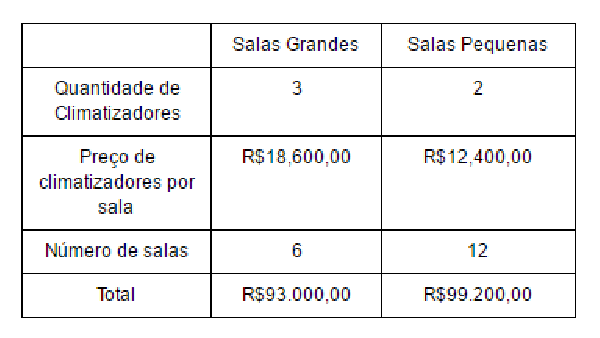
\includegraphics[keepaspectratio=true,scale=1]{figuras/tabela_climatizadores.eps}
\caption{Estimativa de custo dos climatizadores}
\end{figure}

\section{Organização interna}
\subsection{Projeção}
Um dos problemas que o atual prédio de salas de aula da FGA enfrenta é o mau posicionamento dos quadros. Em muitas salas o quadro está muito alto forçando o professor a usar um tablado para alcançar o mesmo e em outras salas está tão baixo que é necessário que o professor só use da metade para cima. Segundo (MORO, 2005) o mobiliário da sala de aula como outros fatores físicos ,são grandes influenciadores no desempenho, segurança, conforto e comportamento dos alunos. Assim (LUZ et al., 2005) afirma que um quadro mal posicionado pode ocasionar o esgotamento dos pequenos músculos ligados aos globos oculares,podendo causar tensão e desconforto em graus mais avançados. 
Desta forma podemos também fazer um comparativo com a posição dos projetores. Muitas vezes quando o professor utiliza o powerpoint, a imagem projetada apresenta baixa nitidez devido a luminosidade que entra pelas janelas e muitas vezes há complicações para enxergar uma parte da imagem que fica entre o quadro e a parede. Outro agravante é a necessidade de subir em carteiras para ligar e desligar esses equipamentos, o que pode comprometer a segurança dos usuários.
Para a questão da projeção da imagem, a solução consiste em colocar a lona de projeção e o projetor em um local da sala cuja luminosidade proveniente das janelas não atrapalhe a imagem projetada. Já para ligar o dispositivo, a solução deste problema é a extensão do mecanismo que liga e desliga o projetor para um local próximo ao professor, onde ficam os cabos que conectam o projetor ao computador.

\subsection{Tablados}
Em grande parte das salas de aula as turmas são muito grandes, então os alunos que escolhem um assento no fundo da sala tem uma dificuldade para enxergar o quadro. A solução para esse problema é a construção de um tablado de madeira com vários níveis similar a um anfiteatro, mas adaptado para as dimensões da sala. Dessa forma, as cadeiras continuarão em sua forma matricial porém, em salas grandes como a Superior 1, o tablado deve surgir a partir da 6ª fileira com degraus de 1 metro de comprimento e 13 centímetros de altura.

\subsection{Tomadas}
Devido ao crescente uso de recursos tecnológicos em sala de aula, tomadas são essenciais. Porém, a localização das tomadas, no fundo e laterais da sala força o aluno que precisa destas, escolher um assento no fundo da sala dificultando sua visão do quadro e do projetor. Para solucionar o problema pode-se incorporar a solução de outro mencionado mais acima. As tomadas podem ser incorporadas ao tablado que será construído para se colocar as carteiras. Assim, pode-se colocar uma tomada perto de cada carteira, aumentando as opções de escolha do lugar onde o alunos deseja se sentar e também a acessibilidade a este recurso.

\subsection{Acústica}
Quanto a acústica, que também é problemática em salas maiores, deverá ser feita a instalação de caixas de som e disponibilização de microfones para os professores. Propõe-se que as caixas de som devam ser instaladas acima do quadro da sala de aula e estará a disposição do professor um microfone para que ele possa ser ouvido por toda a sala.

\subsection{Viabilidade}

\subsubsection{Tomadas e tablados}
O bom desempenho dos alunos está diretamente atrelado ao andamento da aula. Aos alunos que se sentam na frente tem a melhor visão do quadro e consequentemente tem melhor desempenho porém os alunos que estão mais distantes do quadro são prejudicados não só pelo impedimento da visão, mas também de locomoção. Além disso, notou-se a necessidade de realocar as tomadas, para que estejam mais acessíveis aos alunos que não sentam próximos às paredes da sala.
A proposta é a implementação de tablados de madeira que cooperaram para a melhor distribuição dos alunos na sala de aula otimizando o andamento da aula dando visibilidade para todos os alunos presentes, mesmo nas maiores salas. Ainda pensando na comodidade dos alunos o tablado terá em sua estrutura instalação elétrica colocando assim à disposição dos alunos tomadas.
Quanto às dimensões do tablado deverá ter quatro degraus de 1m (um metro) de comprimento 13cm (treze centímetros) de altura e 5m (cinco metros) de largura. 

\begin{figure}[!ht]
\centering
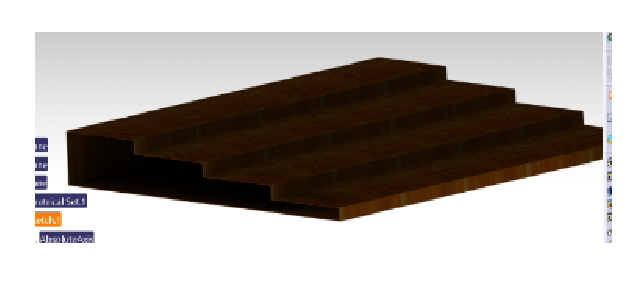
\includegraphics[keepaspectratio=true,scale=1]{figuras/Tablado.eps}
\caption{Esquematização do tablado}
\end{figure}

A viabilidade da implementação do tablado começa pelo orçamento. A superfície do tablado tem 86$m^2$ sendo que no mercado hoje a madeira custa em média R\$ 79,90$m^2$, possuirá 20 tomadas ao custo médio de R\$ 15,00 e 25 metros de fio ao custo de R\$ 4,90 por metro. Sem levar em consideração a estrutura de sustentação do tablado apenas com os materiais o custo de aproximadamente R\$ 7400,00. A mão de obra deverá ser negociada levando em consideração a quantidade. Dessa forma, apesar de ser um custo a mais comparado ao prédio atual, essa solução é somente necessária nas salas grandes como a S1 e é capaz de melhorar o interesse e desempenho dos alunos de forma significativa.

\subsubsection{Equipamentos}
O diferencial dos equipamento é o uso de um quadro panorâmico único e caixas de som. Já para os projetores foi feito um orçamento juntamente com os outros equipamentos. Dessa forma, foi realizada uma pesquisa de mercado para se encontrar os itens citados, que apresentem o melhor custo benefício. As salas maiores para turmas de até 120 alunos receberão o quadro côncavo e dois projetores além da caixa de som. As salas menores e os laboratórios terão apenas um projetor e um quadro branco normal, incluindo uma caixa de som.
O projetor que melhor se adequou às nossas necessidades foi o projetor LED 2200 lumens BT720 da BTEC. É um aparelho bivolt, possui as principais entradas do mercado como HDMI, VGA entre outras, sua lâmpada de projeção é uma lâmpada led o que gera menos consumo de energia e possui uma vida útil maior. Seu preço está em torno de R\$1200.

\begin{figure}[!ht]
\centering
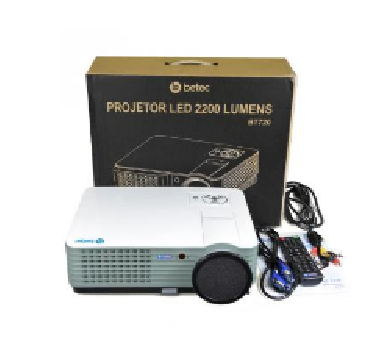
\includegraphics[keepaspectratio=true,scale=1]{figuras/equipamentos.eps}
\caption{Equipamentos}
\end{figure}

O quadro que atende a todas as nossas necessidades é o quadro branco cerâmico da DigiSonic. O seu material possui uma alta resistência a manchas e possuindo ainda propriedades magnéticas podendo usar ímãs no mesmo. Possui uma garantia da superfície de 10 anos. O preço que eles cobram por um quadro simples do mesmo material com tamanho de (1,23 x 1,26) está em torno de R\$399. Segue uma imagem do quadro e uma tabela comparativa com o quadro comum.

\begin{figure}[!ht]
\centering
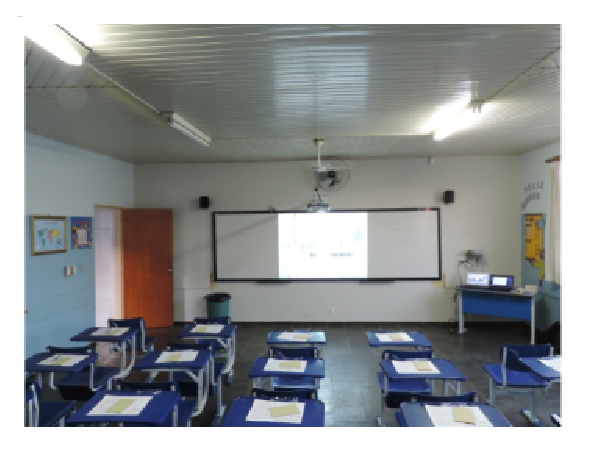
\includegraphics[keepaspectratio=true,scale=1]{figuras/quadro.eps}
\caption{quadro}
\end{figure}

\begin{figure}[!ht]
\centering
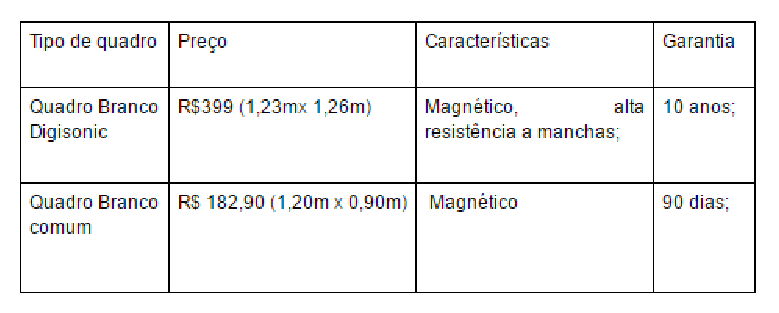
\includegraphics[keepaspectratio=true,scale=1]{figuras/comparativo_precos_quadros.eps}
\caption{Preços do quadro comum x quadro proposto}
\end{figure}

Por fim a caixa de som que atende as necessidades da sala é a TRC 358 por esta possuir conexão bluetooth, permitindo que qualquer aparelho se conecte a mesma, possuindo conexão para microfone sem fio , além de possuir entrada de áudio componente. Inclui também leitor de cartão de memória. Seu preço está em torno de R\$550.

\begin{figure}[!ht]
\centering
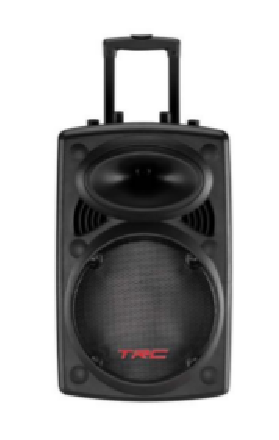
\includegraphics[scale=1]{figuras/caixa_de_som.eps}
\caption{Exemplo de caixa de som}
\end{figure}

Como dito anteriormente cada sala grande receberá um quadro panorâmico, dois projetores e duas caixa de som, o quadro da sala grande tem dimensões de (2.00 x 1.26). Assim o custo dos equipamentos de uma sala grande fica em torno de R\$4148,77. Já a sala pequena recebe apenas um quadro branco normal com as dimensões (1.23 x 1.26) do mesmo material do quadro panorâmico, um projetor e uma caixa de som, desta forma o custo de seus equipamentos fica em R\$2149.

\section{Materiais}
Assim como foi feito nos tópicos anteriores, as propostas de soluções para o uso de materiais diferenciados na construção do Prédio Inteligente são apenas sugestões, visto que os autores do projeto não possuem capacidade para decidir entre um material e outro efetivamente. O conhecimento das propriedades dos materiais auxilia na sua correta seleção para os diversos usos, na determinação das suas propriedades e qualidades tecnológicas, proporciona a escolha de fatores de segurança adequados e vários outros fatores que que irão influir de maneira decisiva na parte econômica de um projeto.
A partir disso nota-se que é fundamental a seleção de materiais que serão utilizados no projeto. Uma metodologia comumente usada para a seleção de materiais na fase inicial é a Metodologia de Pugh. Essa metodologia consiste em comparar os diversos conceitos de produto com que se pretende trabalhar com um conceito de referência facilitando a escolha de um conceito que se sobressaia.
É feita então, uma análise das vantagens (ou pontos positivos), desvantagens (ou pontos negativos) e equivalência dos conceitos propostos em relação ao conceito de referência. Esta técnica possibilita a escolha do melhor conceito, chamado de conceito “vencedor”, a ser adotado para o produto. A seguir, tem-se o comparativo entre as características dos materiais que embora comumente utilizados, foram descartados do projeto e os materiais que foram escolhidos para suprir uma maior cota de requisitos de um prédio inteligente e sustentável.

\begin{figure}[!ht]
\centering
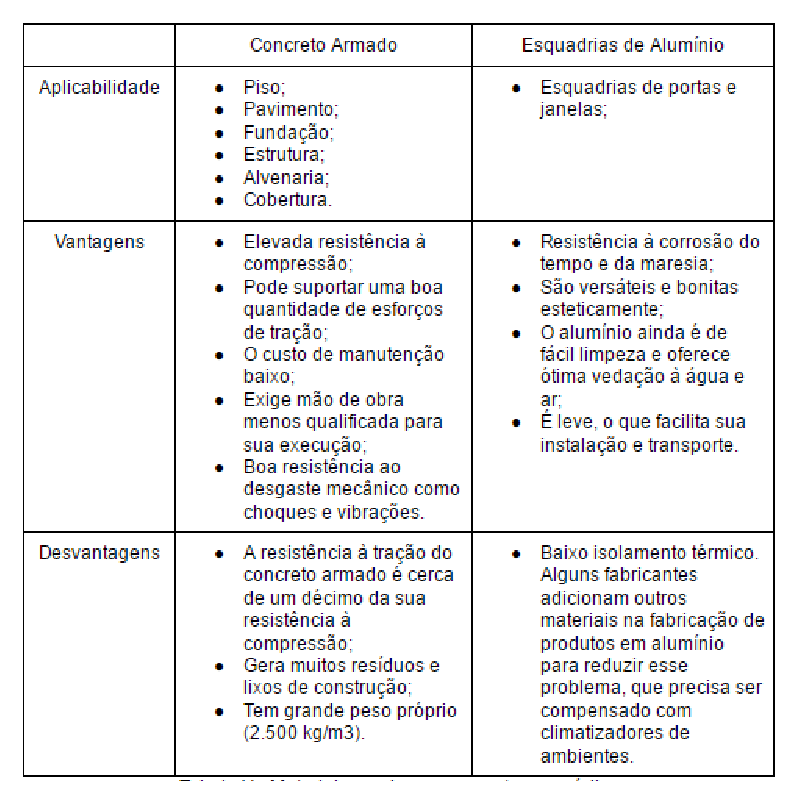
\includegraphics[keepaspectratio=true,scale=1]{figuras/materiais_usados_comumente_em_predios.eps}
\caption{Materiais usados comumente em prédios}
\end{figure}

\begin{figure}[!ht]
\centering
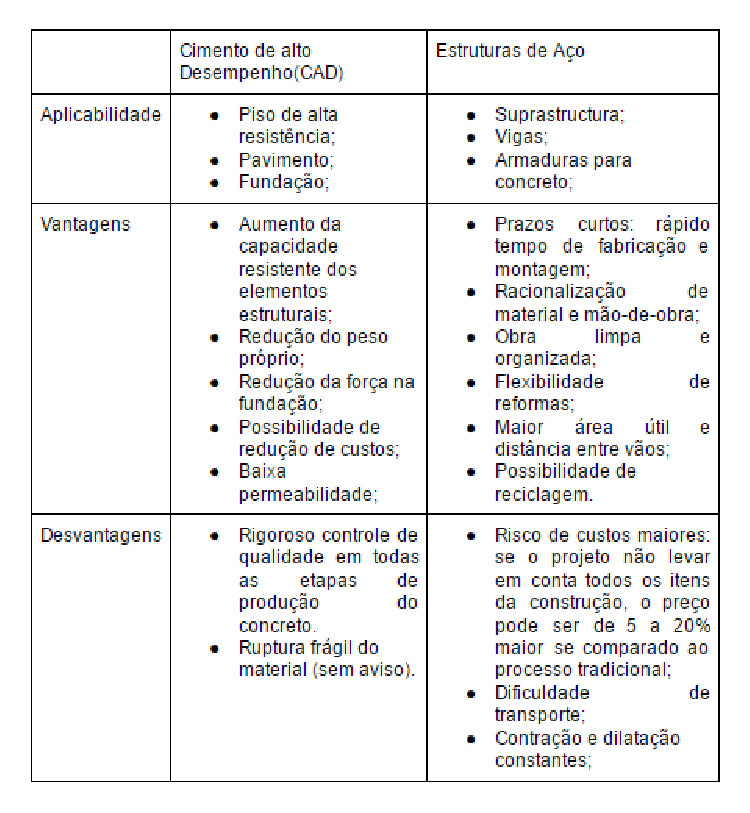
\includegraphics[keepaspectratio=true,scale=1]{figuras/vantagens_e_desvantagens_material1.eps}
\caption{ Vantagens e desvantagens dos materiais sugeridos 1}
\end{figure}

\begin{figure}[!ht]
\centering
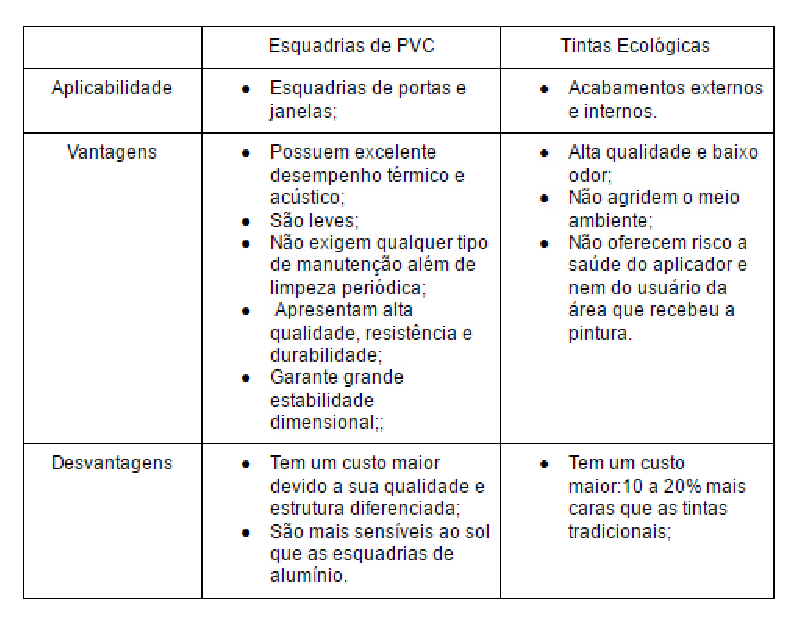
\includegraphics[scale=1]{figuras/vantagens_e_desvantagens_do_material_2.eps}
\caption{ Vantagens e desvantagens dos materiais sugeridos 2}
\end{figure}

Para a cobertura, uma alternativa moderna e econômica são as lajes nervuradas. Podem ser feitas com concreto ecológico e sua forma geométrica reduz o consumo de aço e concreto em até 30\%, diminuído também o peso total da estrutura.
Com o recente senso de responsabilidade ecológica e a aplicação dos conceitos de sustentabilidade na construção civil, diversos materiais estão sendo desenvolvidos buscando ser mais eficientes e menos agressivos ao ambiente. No entanto, poucas opções estão disponíveis no mercado ou são produzidos em larga escala, o que torna esses materiais inviáveis ao projeto. Dessa maneira em alguns casos, ainda que existam soluções mais tecnológicas e avançadas, foi necessário se ater a materiais que favorecem disponibilidade, custo e fácil manuseio.

\subsection{Viabilidade}

A tabela a seguir possui um valor estimado para o concreto armado e um tipo de CAD para o ano de 2012, fornecidos pela Gerência de Composições de Custos e Preços da SANAEGO.

\begin{figure}[!ht]
\centering
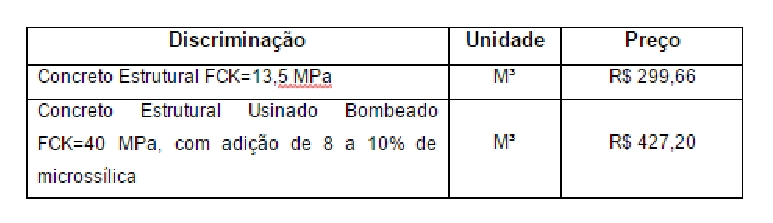
\includegraphics[keepaspectratio=true,scale=1]{figuras/tabela_com_precos_concreto.eps}
\caption{  Preços dos concretos comparados
}
\end{figure}

Nota-se que o CAD chega a ser 29,85\% mais caro que o concreto armado, todavia as características de durabilidade e da possibilidade da redução na largura e na quantidade de pilares do CAD fazem dele uma opção com melhor custo benefício. Um exemplo disso é o edifício E-Tower em São Paulo onde o CAD foi a solução técnico-econômica apresentada, em decorrência da necessidade de se reduzir as dimensões dos pilares da fachada Norte que apresentavam elevada carga nos subsolos.

\begin{figure}[!ht]
\centering
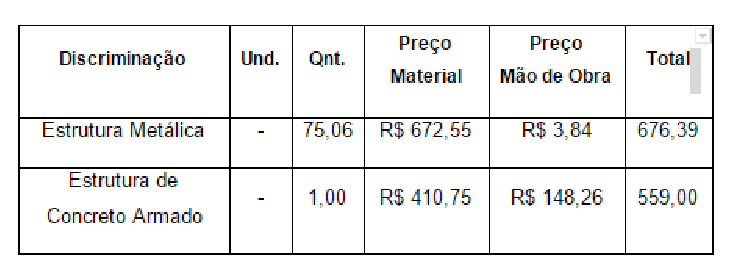
\includegraphics[keepaspectratio=true,scale=1]{figuras/precometais.eps}
\caption{Custo do metais utilizados}
\end{figure}

Apesar de a estrutura metálica ter um custo mais alto, o emprego desse material possui outras vantagens que viabilizam sua utilização. De acordo com a Brandão \& Marmo Engenharia e Construções o aço estrutural foi selecionado em função da importância do cumprimento de um curto prazo de obra e pilares de seções reduzidas em relação à solução em concreto, fundamental para os conceitos e pré-requisitos de estética e layout do projeto.

\begin{figure}[!ht]
\centering
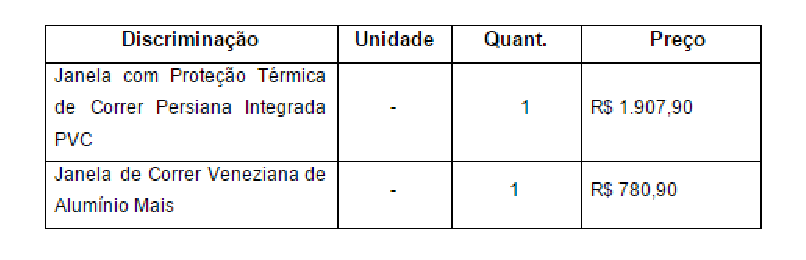
\includegraphics[keepaspectratio=true,scale=1]{figuras/precojanelas.eps}
\caption{Custo das janelas a serem utilizadas}
\end{figure}

A pesquisa mostra que a esquadria de PVC é aproximadamente 60\% mais cara que a de alumínio. Após uma análise de custo benefício, levando em conta os requisitos do projeto, conclui se que apesar das inúmeras vantagens do PVC, a esquadria de alumínio se adaptaria melhor ao orçamento.

\begin{figure}[!ht]
\centering
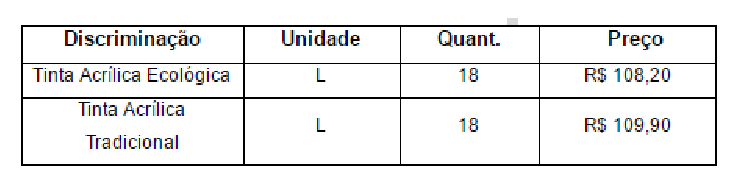
\includegraphics[scale=1]{figuras/custotintas.eps}
\caption{Custo das tintas utilizadas}
\end{figure}
\indent

Constata-se que a tinta ecológica, além de possuir diversas vantagens qualitativas, também oferece um menor custo, tornando ela uma ótima solução para o projeto.

\chapter[Smart Grid]{Smart Grid}
No sistema de geração solar fotovoltaica, os principais dispositivos necessários para a instalação da mini-usina são os descritos abaixo alguns dos dispositivos foram alterados devido não ter certificação INMETRO, foi substituído por dispositivos semelhantes e que substituem com a mesma funcionalidade. OS dispositivos alterados foram a placas canadian de 255w pela placa da mesma marca com 260w o outro dispositivo foi o inversor ABB de 50KW que foi alterado pelo inversor da WEG de 20Kw.
\textbf{Módulos fotovoltaicos:}Módulos fotovoltaicos: usados para converter a energia luminosa em energia elétrica. O módulo fotovoltaico escolhido para a instalação da mini-usina foi o da marca Canadian, certificado pelo INMETRO pelo número de registro 000581/2016, e possui as características descritas pela figura ~\ref{fig:caracteristica_fotovoltaico_1}.

\begin{figure}[!ht]
  \centering
  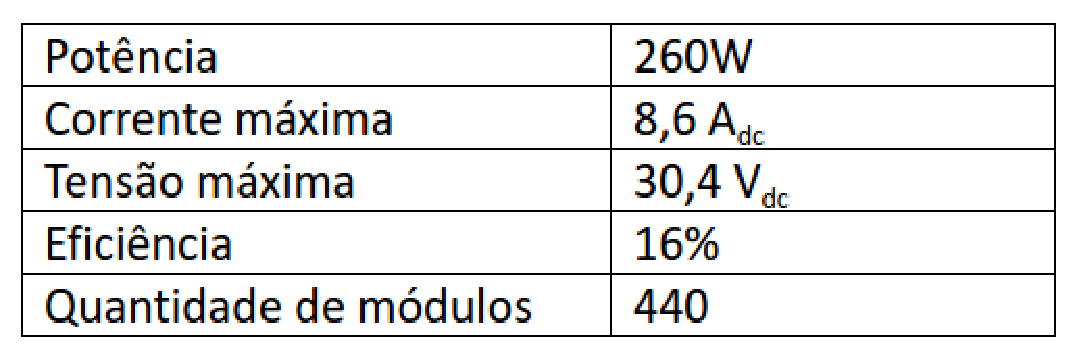
\includegraphics[keepaspectratio=true,scale=0.6]{figuras/caracteristicas_fotovoltaico.eps}
  \caption{Características do Módulo Fotovoltaico}
  \label{fig:caracteristica_fotovoltaico_1}
\end{figure}

\textbf{Inversores:} dispositivos que transformam a energia de corrente contínua oriunda dos módulos fotovoltaicos em corrente alternada. O inversor escolhido foi o SIW600 T20-44 da WEG, certificado pelo INMETRO pelo número de registro 000078/2017, sendo que suas principais características descritas pela figura ~\ref{fig:caracteristica_fotovoltaico_2}.

\begin{figure}[!ht]
  \centering
  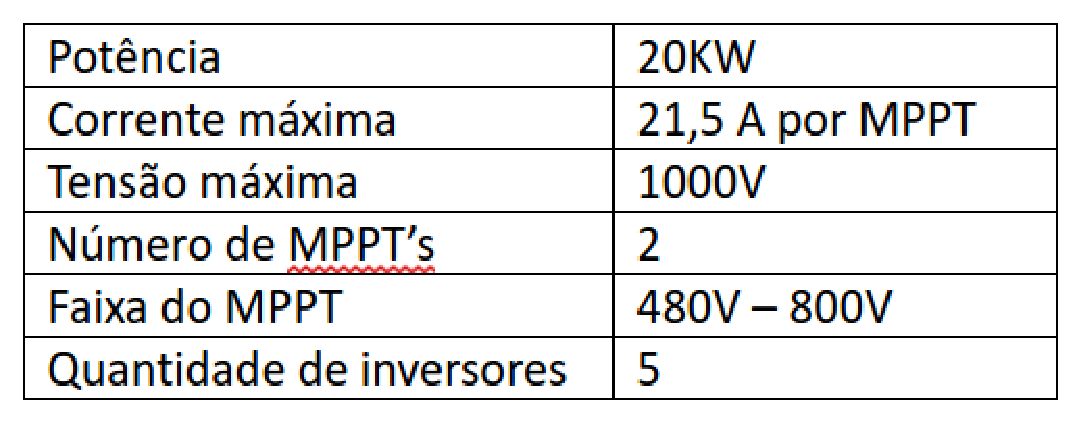
\includegraphics[keepaspectratio=true,scale=0.6]{figuras/SmartGrid_Caracteristicas_fotovotaico_2.eps}
  \caption{Características do Inversor}
  \label{fig:caracteristica_fotovoltaico_2}
\end{figure}

\begin{figure}[!ht]
  \centering
  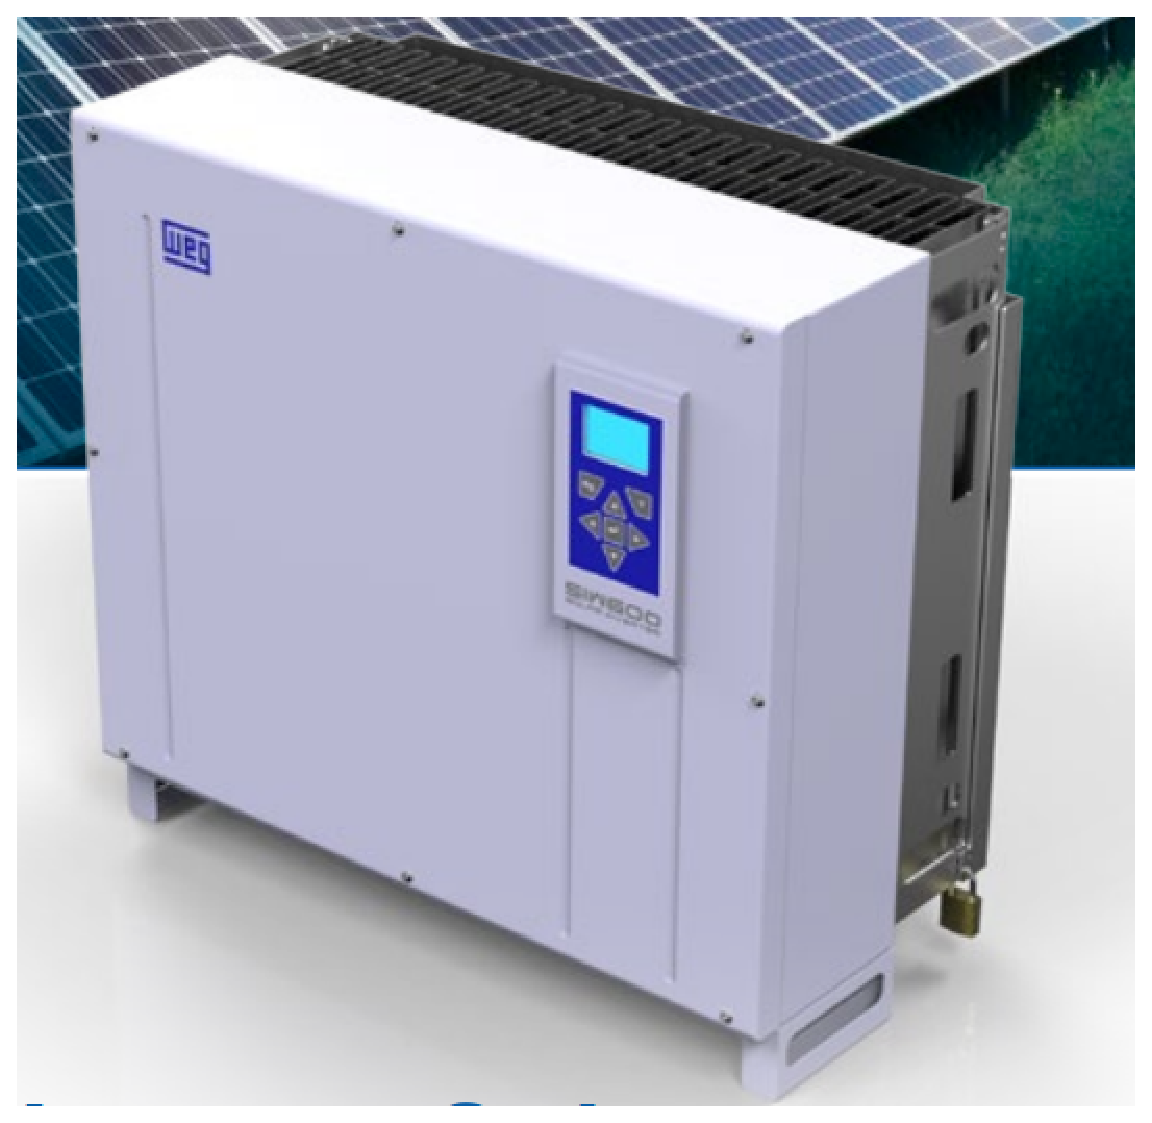
\includegraphics[keepaspectratio=true,scale=0.4]{figuras/inversor.eps}
  \caption{Inversor}
  \label{fig:inversor}
\end{figure}

\textbf{String Box:} Caixa que contém disjuntores que servem como chaves e dispositivos de proteção como DPS e fusíveis. São necessários 5, uma para cada inversor, sendo que a mesma é conectada antes deste.
\textbf{Multimedidores de energia:} dispositivos usados para a medição de energia consumida e gerada para cada conjunto de módulos fotovoltaicos e inversor. Ou seja, é instalado um multimedidor após cada inversor, para o caso específico serão usados 5 desses dispositivos.
\textbf{Medidor bidirecional:} dispositivo usado para medir o consumo de energia do prédio e a energia gerada inserida na rede. Este é um relógio de faturação e é instalado pela distribuidora (CEB, no caso de Brasília).
\textbf{Suporte para laje:} dispositivo instalado na laje para dar suporte aos módulos fotovoltaicos. O mesmo é constituído de um perfil em “ L “, que fornece inclinação e sustentação para os painéis e por um suporte estruturado que fornece apoio e que aguente o peso do painel. O suporte deve ser de alumínio inoxidável e galvanizado pois o mesmo ficará exposto ao sol e chuva. 
\textbf{Grampos de fixação:} dispositivos usados para prender os painéis no suporte.
\textbf{Conectores MC4:} conectores inseridos no final de cada cabo, usados para conectar os módulos fotovoltaicos entre si.
\textbf{Cabos:} usados para fazer a conexão dos dispositivos.

\section{Instalação do Sistema Solar Fotovoltaico}

Para a instalação do sistema de geração, os dispositivos são dispostos como segue:
\begin{itemize}
  \item Primeiramente monta-se os suportes de alumínio na lage;
  \item Em seguida os painéis fotovoltaicos são fixados no suporte com os grampos de fixação;
  \item Os painéis são conectados entre si em série e/ou em paralelo;
  \item Dois fios, sendo um positivo e um negativo, saem do conjunto de painéis e são ligados na string box;
  \item Na saída da string box saem também dois fios que são conectados no inversor de frequência;
  \item Na saída do inversor saem 3 fios (sistema trifásico) que são conectados nos multimedidores e no quadro geral da instalação elétrica do prédio;
  \item Por fim, o medidor bidirecional é instalado e conectado no quadro geral para faturação da energia consumida e gerada.
\end{itemize}

A Figura ~\ref{fig:fluxograma}, mostra um fluxograma geral da instalação do sistema solar fotovoltaico.

\begin{figure}[!ht]
  \centering
  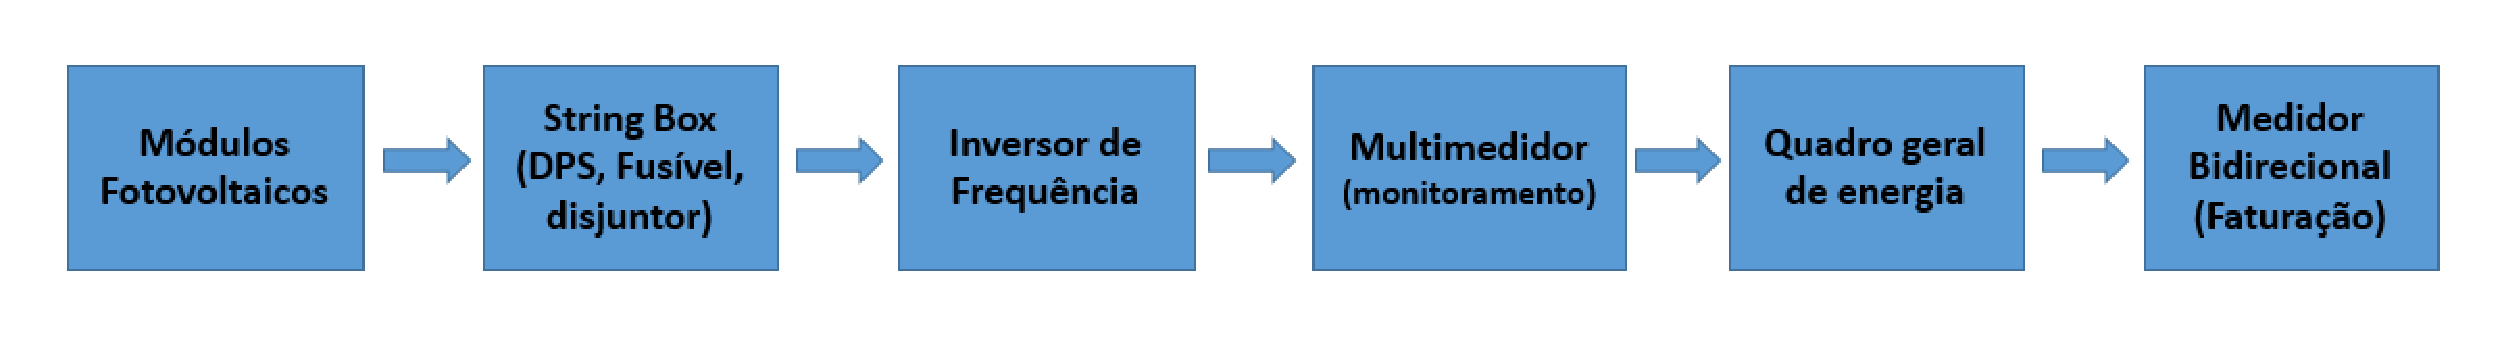
\includegraphics[keepaspectratio=true,scale=0.4]{figuras/instalacao_sistema.eps}
  \caption{Fluxograma geral da instalação do sistema solar fotovoltaico}
  \label{fig:fluxograma}
\end{figure}

\section{Manutenção}
Diante da constante busca por uma energia cada vez menos poluente, o uso de placas fotovoltaicas se apresenta como uma excelente alternativa sustentável, proporcionando economia nos gastos elétricos e produção de uma energia mais limpa. No entanto, esse modo de geração de energia demanda uma certa atenção no que diz respeito à manutenção do sistema.
Especialistas concordam que painéis solares sujos não produzem tanta energia quanto painéis limpos. Essa perda pode chegar até 25\% em alguns casos, de acordo com o laboratório Nacional de Energias Renováveis dos Estados Unidos (NREL)
Em regra geral, as informações são de realizar a limpeza e manutenção de placa solar anualmente. Porém, em lugares com muita incidência de poeira, como no caso da FGA, é indicada a limpeza a cada 4 meses.A inspeção da parte elétrica do Sistema Fotovoltaico acontece igual a inspeção elétrica comum, fazendo uma inspeção visual. A limpeza pode ser feita com um jato de água ou até mesmo com uma vassoura de cerdas macias. No entanto como a área do prédio da Fga é grande, o interessante é a instalação de um sistema de monitoramento para manter vigilância sobre o desempenho de seus painéis solares.
Um equipamento que auxilia bastante no momento de identificar possíveis problemas no sistema fotovoltaico são os loggers, que servem para o monitoramento do sistema. É possível verificar o quanto de energia está sendo produzido e outros parâmetros do sistema, permitindo verificar se o equipamento está funcionando corretamente, assim quando o desempenho cair, você saberá que a manutenção é faz necessária.  
Algumas vantagens de instalar um sistema de monitoramento do painel solar são:

\begin{itemize}
  \item Acompanhar quanta energia está sendo produzida por seus painéis solares.
  \item Os sistemas de monitorização podem mostrar como o usuário está beneficiando o meio ambiente, como os valores mais baixos de emissões de CO2 em comparação com outros sistemas de energia. Essas estatísticas podem ajudá-lo a obter benefícios fiscais no preenchimento da declaração de imposto de renda.
  \item Diagnosticar problemas através do sistema de monitoramento. Muitos destes dispositivos irá  dizer quais as áreas do painel solar não estão funcionando corretamente e precisam de reparo.
  \item Possibilidade de ter  informações sobre os  painéis solares em um display de parede no próprio local ou através da Internet, para ter acesso sem ser no Campus da Fga.
\end{itemize}

\section{Monitoramento das Placas Fotovoltaicas}

\begin{figure}[!ht]
  \centering
  \includegraphics[keepaspectratio=true,scale=0.3]{figuras/DataLogger.eps}
  \caption{DataLogger Meteo-40S M11010}
  \label{fig:datalogger}
\end{figure}

\begin{figure}[!ht]
  \centering
  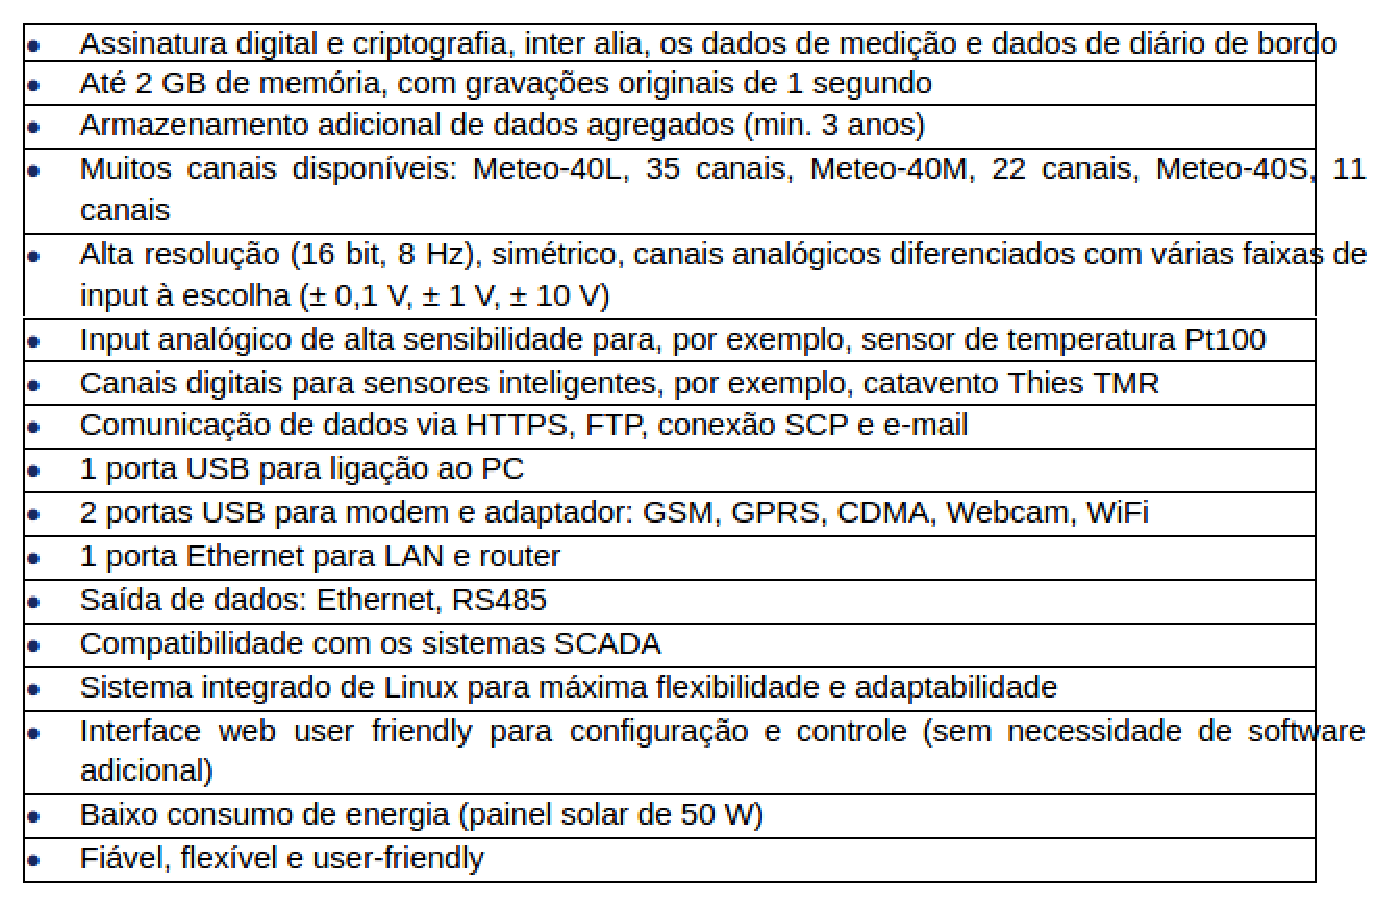
\includegraphics[keepaspectratio=true,scale=0.5]{figuras/SmartGrid_Monitoramento_placas_fotovotaicas_1.eps}
  \caption{DataLogger Meteo-40S M11010}
  \label{fig:tabela_datalogger_1}
\end{figure}

\begin{figure}[!ht]
  \centering
  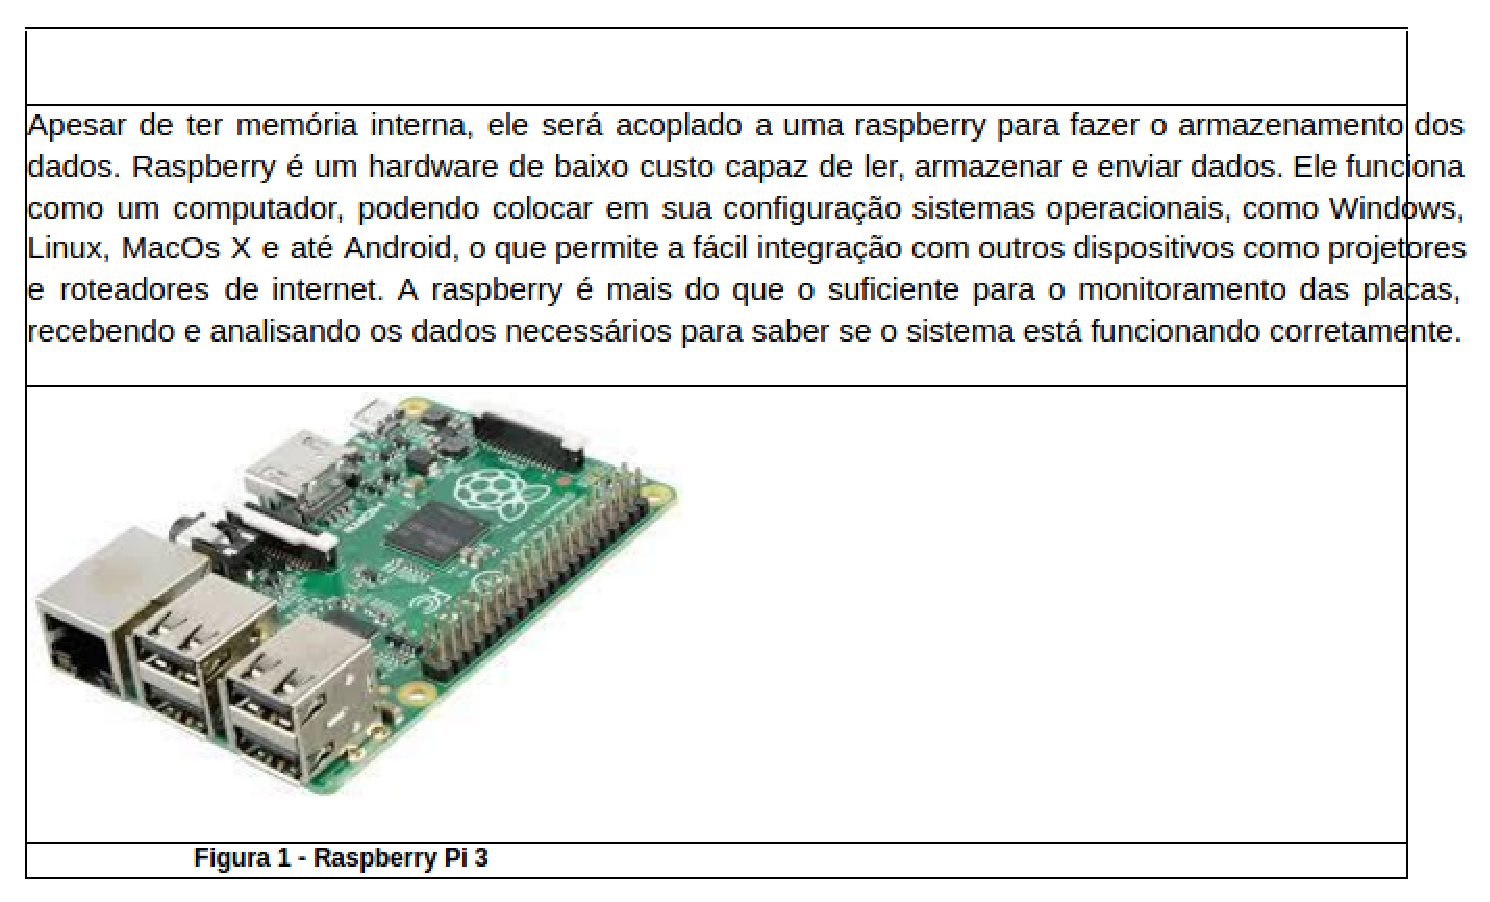
\includegraphics[keepaspectratio=true,scale=0.5]{figuras/SmartGrid_Monitoramento_placas_fotovotaicas_2.eps}
  \caption{DataLogger Meteo-40S M11010}
  \label{fig:tabela_datalogger_2}
\end{figure}

\section{Reciclagem das Placas}

A vice presidente Lisa Krueger, da First Solar, maior fabricante de painéis solares do mundo, afirma , que até 97 por cento dos materiais utilizados na produção dos módulos solares podem ser extraídos e reaproveitados utilizando reciclagem térmica. Porém esse recurso só pode ser utilizado nos módulos sem silício em sua composição.
Já as placas com silício devem ser divididas manualmente ou mecanicamente. A reciclagem mecânica envolve a remoção de cada componente do painel solar, salvando e reutilizando alguns materiais, podendo chegar até a revenda.  É um processo quimicamente menos eficiente do que a reciclagem térmica , mas ainda apresenta resultados acima de 95\%.

\subsection{Viabilidade}
Visto que a energia solar está bem consolidada no Brasil tem-se como conclusão que a viabilidade do sistema fotovoltaico,mesmo com um preço razoavelmente alto como mostrado na tabela abaixo.As placas solares tem uma vida útil de 25 anos e como foi descrito a manutenção é relativamente simples, esses pontos facilitam quando deseja-se escolher uma forma de produzir energia sustentável.O custo de instalação é bem alto,porém a conta de energia da FGA é muito cara, custando cerca de R\$40.000,00 (foi solicitado a conta de energia atual,porém não foi possível a aquisição da mesma, dessa forma esse valor é um valor que se aproxima da conta de energia mensal da FGA atual,de acordo com a conta que estará em anexo) de acordo com o dimensionamento feito serão necessários 440 módulos fotovoltaicos para que supra a quantidade energética de 23.000 kwh/mês isto é aproximadamente a metade de energia gasta pela FGA dessa forma a conta energética de 1 prédio se reduziria a R\$20.000,00 visto que as estimativas feitas por um prédio consome a metade.Lembrando que não será possível pagar, “descontar”, os 40 mil reais de energia devido a demanda contratada, que para 1 prédio é por volta de R\$8,200,00 dessa forma a economia se dá pelo restante ou seja R\$ 11.800,00. Assim,considerando que as placas gerem os 23.000kwh/mês o sistema fotovoltaico se paga em um tempo aproximado  de 2 anos e 7 meses.Conclui-se que têm -se um custo benefício devido a longevidade dos sistema fotovoltaicos visto que em 25 anos têm-se uma economia aproximada de R\$3.174.200.

\begin{figure}[!ht]
  \centering
  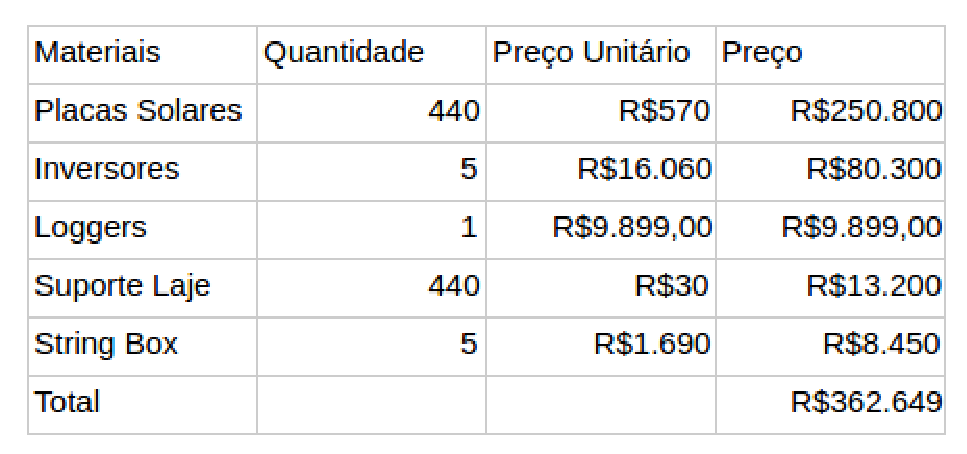
\includegraphics[keepaspectratio=true,scale=0.6]{figuras/SmartGrid_Tabela_de_Custos.eps}
  \caption{Tabela de Custos}
  \label{fig:tabela_custos}
\end{figure}

\section{Gerador Movido a Biodisel}
Considerando que o gerador à biodiesel será usado apenas em casos de emergência, ou seja, quando houver queda de energia fornecida pela Companhia Energética de Brasília (CEB), e que o dimensionamento necessário já foi feito no Ponto de Controle 2 para um gerador à diesel.
Para o prédio, dimensionou-se um gerador de 155,10 kW, porém o modelo comercial encontrado mais próximo foi o gerador à diesel modelo C170D6 de 170 kW e 212 kVA (para operação em standby\footnote{Operação Standby: acionado em casos de emergência.}), motor do tipo 6CTA 8.3-G2, visualizado na Figura 01. Ou seja, o gerador comercial mais próximo encontrado está superdimensionado em 8,77\%, o que podemos considerar como um fator de segurança.

\begin{figure}[!ht]
  \centering
  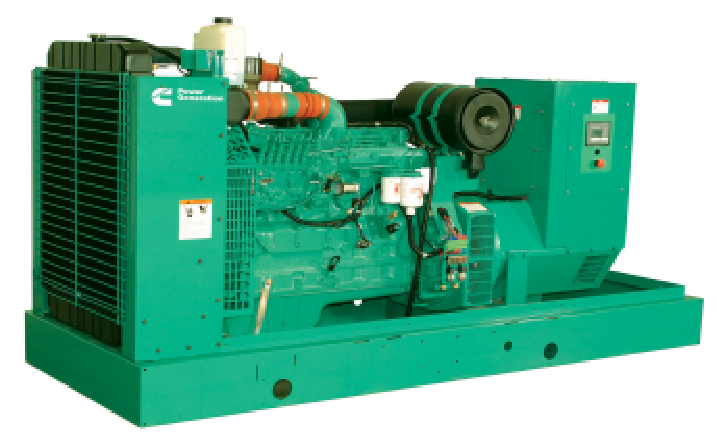
\includegraphics[keepaspectratio=true,scale=0.6]{figuras/gerador.eps}
  \caption{Gerador C170D6}
  \label{fig:gerador}
\end{figure}

Nós entramos em contato diversas vezes com duas empresas fornecedoras de geradores, a STEMAC e GELEC ENERGY, porém a primeira não nos retornou e a segunda apresentou apenas seu portfólio de produtos, mas não as especificações técnicas e preços dos mesmos, inclusive do gerador à biodiesel que requeremos para o hipotético projeto na Faculdade do Gama da Universidade de Brasília (FGA/UnB).
Devido à dificuldade da obtenção dos preços do gerador à diesel, foi feita outra busca para geradores similares a fim de obter um custo desses produtos, e com base nisso foi encontrado um gerador à diesel de modelo Toyama TDMG125SE3 de 125 kVA com preço de R\$ 54.685,09 no site da loja NOWAK, porém serão necessários dois geradores deste modelo, totalizando 250 kVA, isto é, o projeto agora fica superdimensionado em 15,2\%, recordando que podemos usá-lo como fator de segurança. Na Figura ~\ref{fig:gerador2} podemos ver o gerador mencionado e na tabela da figura ~\ref{fig:gerador2_tabela} seus dados técnicos.

\begin{figure}[!ht]
  \centering
  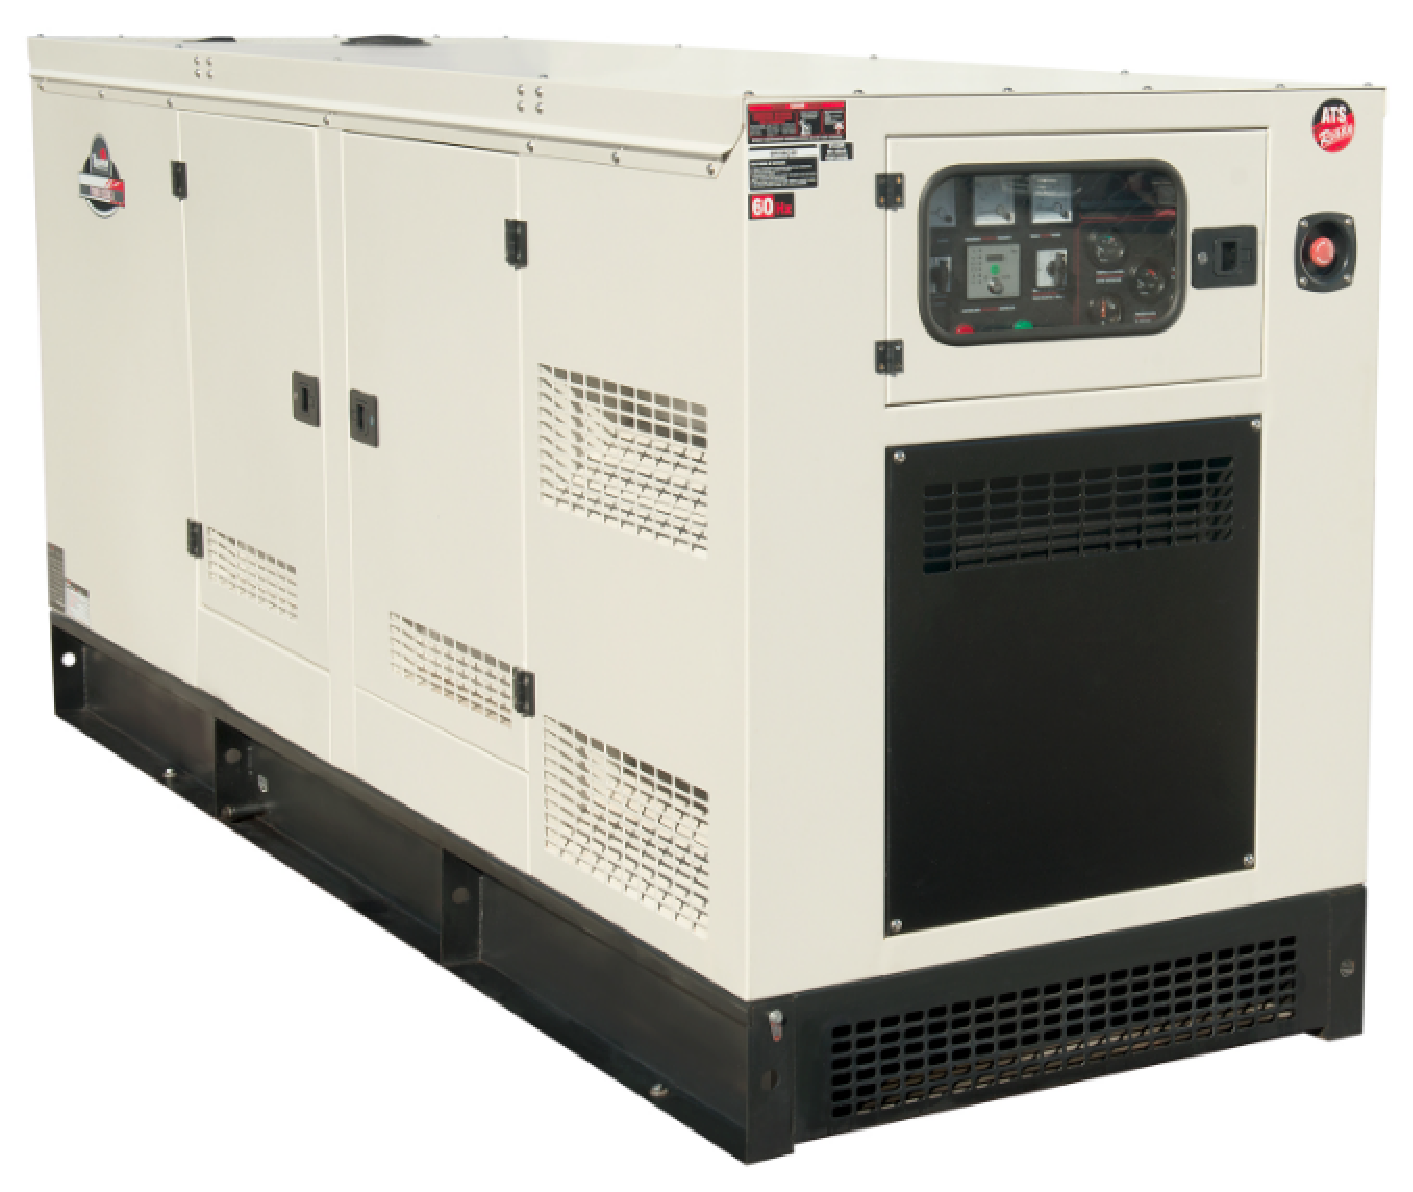
\includegraphics[keepaspectratio=true,scale=0.2]{figuras/gerador2.eps}
  \caption{Gerador Toyama TDMG125SE3}
  \label{fig:gerador2}
\end{figure}

\begin{figure}[!ht]
  \centering
  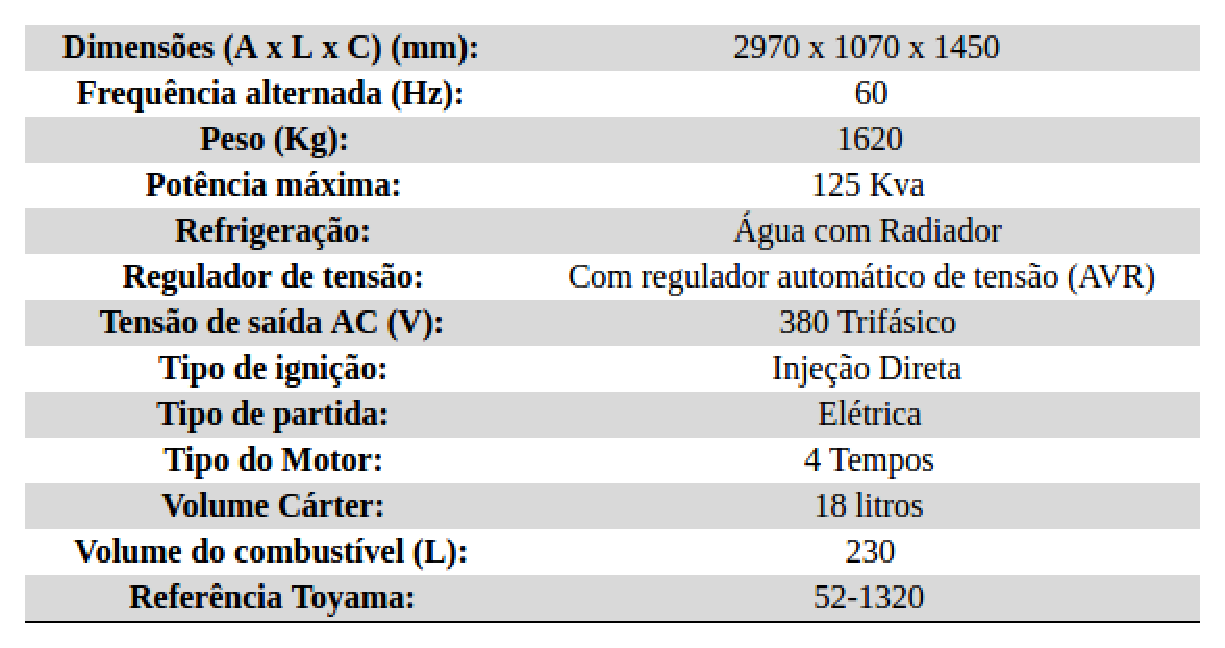
\includegraphics[keepaspectratio=true,scale=0.4]{figuras/SmartGrid_Dados_gerador_biodisel.eps}
  \caption{Dados Técnicos - Gerador Toyama TDMG125SE3}
  \label{fig:gerador2_tabela}
\end{figure}

\chapter[Controle de Acesso]{Controle de Acesso}
\section{Escolha da Tecnologia}
A área de Controle de Acesso está aqui subdividida em três grandes principais frentes tecnológicas.
São elas: controle da entrada do estacionamento privativo, controle da entrada em salas e laboratórios
e, por fim, controle de frequência durante as aulas.

Dentre essas frentes, foram elegidas três possibilidades diferentes para a inserção na Universidade.
A tabela a seguir elicita-as, bem como apresenta as vantagens e desvantagens para cada um dos casos.

\begin{table}[h]
  \centering
  \caption{Tecnologias de Controle de Acesso - Vantagens x Desvantagens}
  \label{my-label}
  \begin{tabular}{|l|l|l|}
    \hline
    \multicolumn{1}{|c|}{\textbf{Tecnologia}} & \multicolumn{1}{c|}{\textbf{Vantagens}}                                                                         & \multicolumn{1}{c|}{\textbf{Desvantagens}}                                                                                                            \\ \hline
    Leitor biométrico                         & \begin{tabular}[c]{@{}l@{}}- Difícil de burlar \\ - Confiável\end{tabular}                                      & \begin{tabular}[c]{@{}l@{}}- Pode gerar falhas na leitura \\ - Não reconhecer uma \\ digital cadastrada\\ - Sistema caro\\ - Sistema frágil\end{tabular} \\ \hline
    Leitor facial/ Leitor de íris             & \begin{tabular}[c]{@{}l@{}}- Difícil de burlar \\ - Confiável\end{tabular}                                      & \begin{tabular}[c]{@{}l@{}}- Sistema de implementação\\ cara\\ - Demora para análise de \\cada pessoa\\ - Risco de furto\\ - Frágil\end{tabular}          \\ \hline
    Leitor RFID                               & \begin{tabular}[c]{@{}l@{}}- Fácil de utilizar\\ - Difícil de burlar\\ - Único para cada estudante\end{tabular} & \begin{tabular}[c]{@{}l@{}}- Custo extra para a \\faculdade\\ - Risco de perda do \\documento\end{tabular}                                                \\ \hline
  \end{tabular}
\end{table}

Apesar de todas as tecnologias sugeridas apresentarem vantagens e desvantagens, o sistema RFID foi o escolhido para atender
a demanda. Esta escolha se deu em virtude deste ser mais eficaz, eficiente e mais acessível financeiramente em relação aos
outros.

\subsection{Breve Descrição da Tecnologia RFID}
O sistema funciona RFID (do inglês \textit{Radio-Frequency IDentification}) é um tecnologia que permite identificação automática
 através de sinais de rádio. Neste projeto será implementado de  por meio de um chip dentro de um cartão, armazenando o
 nome e matrícula do aluno dono do documento e sempre que o documento for apresentado, seus dados serão apresentados nos
 display dos equipamentos. Levando em conta que tanto alunos como professores serão portadores deste documento com chip,
 para o alunos o cartão será utilizado como carteirinha, e para os professores como crachá.

Apesar de todo o grupo de controle de acesso utilizar esta ferramenta, cada uma das frentes utiliza o sistema de forma
diferente e com aparelhos diferentes. Desta forma, cada área tem suas particularidades de funcionamento e regras, como será
 mostrado e explicado a seguir.

\section{Controle de Frequência}
Para o controle de frequência nas aulas, será utilizado o seguinte aparelho (apresentado anteriormente no Ponto de Controle 1).
O funcionamento dele acontece independente de sinal de WiFi e o aparelho é de porte único do professor.

\begin{figure}[!ht]
  \centering
  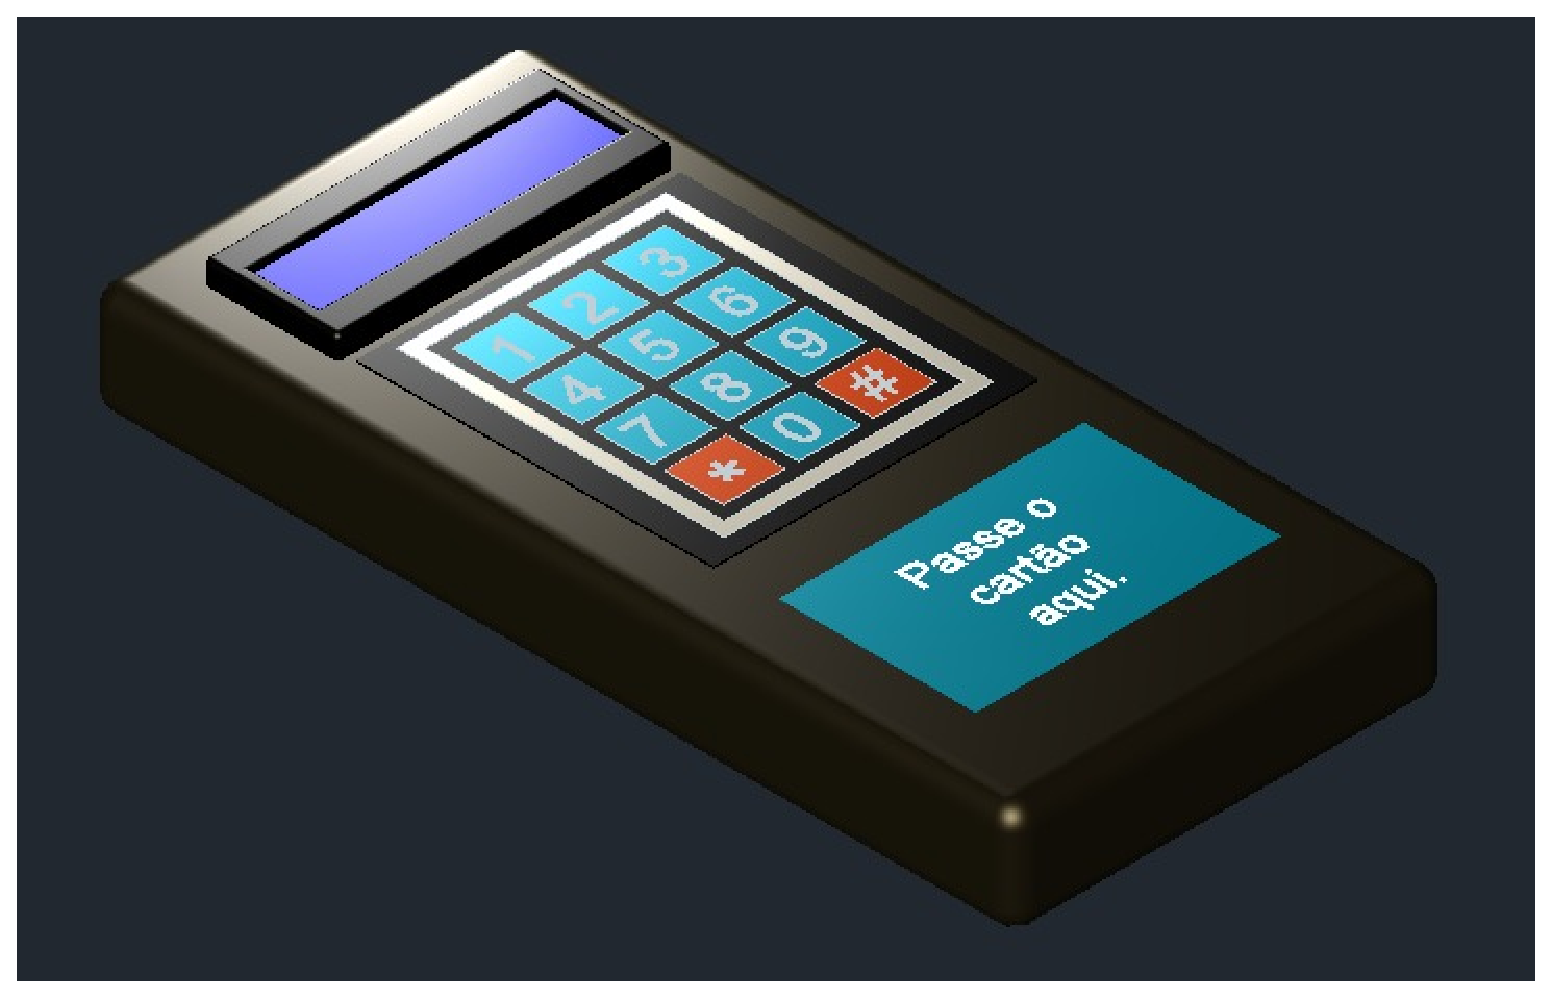
\includegraphics[keepaspectratio=true,scale=0.45]{figuras/freq.eps}
  \caption{Aparelho Para Controle de Frequência}
\end{figure}

Em relação à aspectos técnicos do aparelho, a figura a seguir mostra detalhadamente quais os instrumentos utilizados.

\begin{figure}[h]
  \centering
  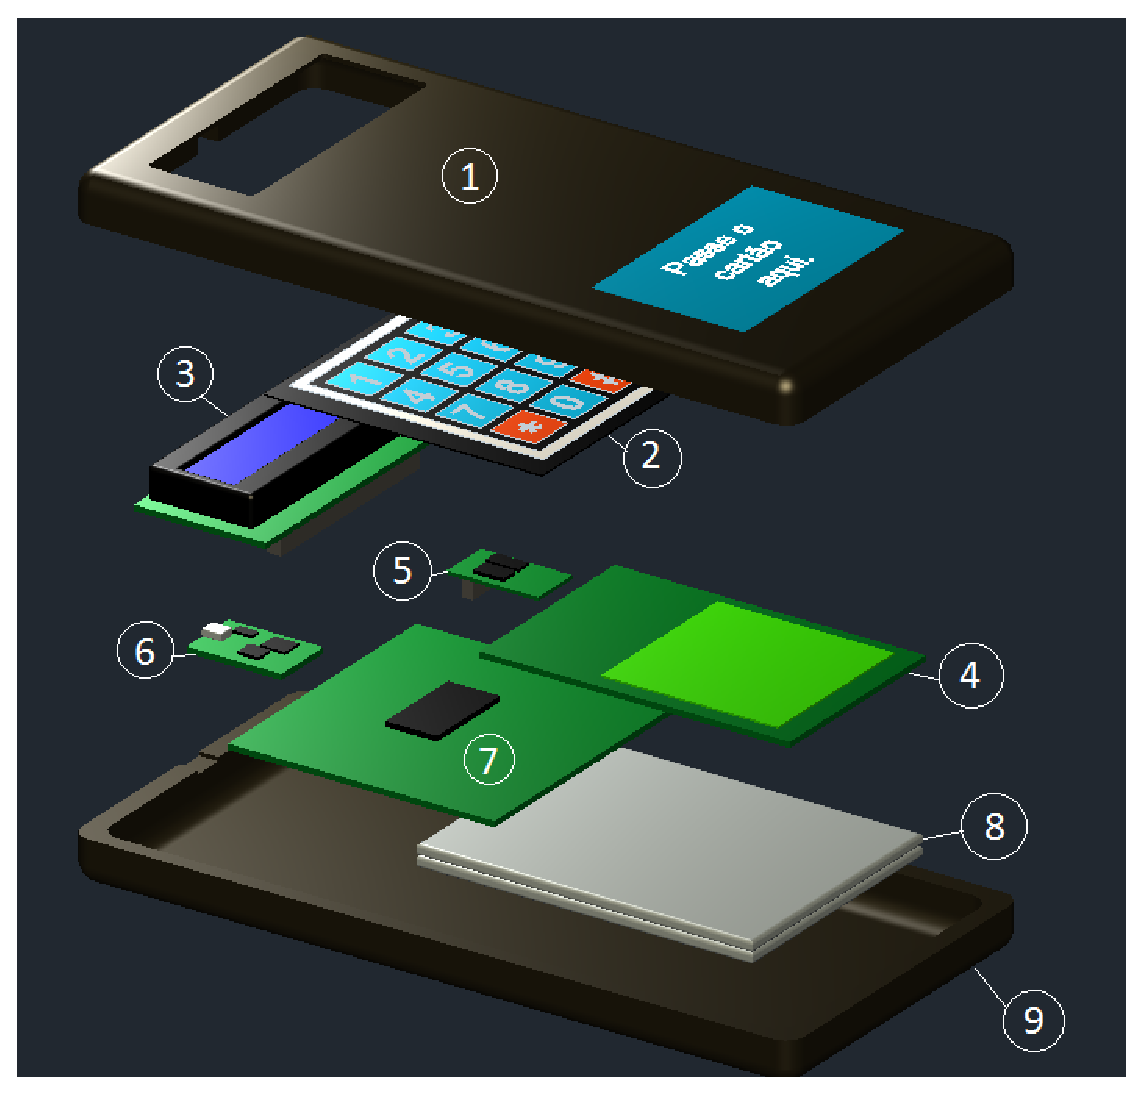
\includegraphics[keepaspectratio=true,scale=0.45]{figuras/aberto.eps}
  \caption{Aparelho Para Controle de Frequência Detalhado}
\end{figure}

Cada um dos componentes possui sua função individual:
\begin{itemize}
  \item Componentes 1 e 9: Case superior e inferior. Há um orifício na parte superior do dispositivo para passagem do conector USB.
  \item Componente 2: Teclado matricial de película 12 teclas.
  \item Componente 3: Display LCD 16x2 com backlight
  \item Componente 4: módulo Leitor de cartões RFID Mfrc522 Mifare, faz leitura e escrita em cartões RFID.
  \item Componente 5: Módulo WiFi ESP8266 ESP-01, se conecta com a rede wifi e transmite e recebe dados servidor online.
  \item Componente 6: Módulo Carregador de Baterias de Lítio TP4056, carrega a bateria através do seu conector USB.
  \item Componente 7: Placa controladora faz as conexões com os demais componentes e possui um microcontrolador ATmega1280 16au da família AVR com o bootloader do Arduino mega.
  \item Componente 8: Baterias do tablet Dl Lenoxx Navcity Phaser. Possuem capacidade de 2000mAh e tensão de 3,7v.
\end{itemize}

Cada um desses microcomponentes têm funções específicas que garantem o funcionamento adequado do instrumento. Sob uma ótica mais específica temos:

\subsection{Kit Módulo Leitor Rfid Mfrc522 Mifare}


Este módulo leitor RFID baseado no chip MFRC522 da empresa NXP é altamente utilizado em comunicação sem contato a uma frequência de 13,56MHz. Este chip, de baixo consumo e pequeno tamanho, permite sem contato ler e escrever em cartões que seguem o padrão Mifare, muito usado no mercado.

Este leitor RFID possui as ferramentas para um projeto de controle de acesso ou sistemas de segurança a um ótimo preço.

Este componentes vai ser conectado a o microcontrolador através dos pinos especiais sda(pino 44), sck(pino 20), miso(pino 22) e mosi(pino 21).

\begin{figure}[!ht]
  \centering
  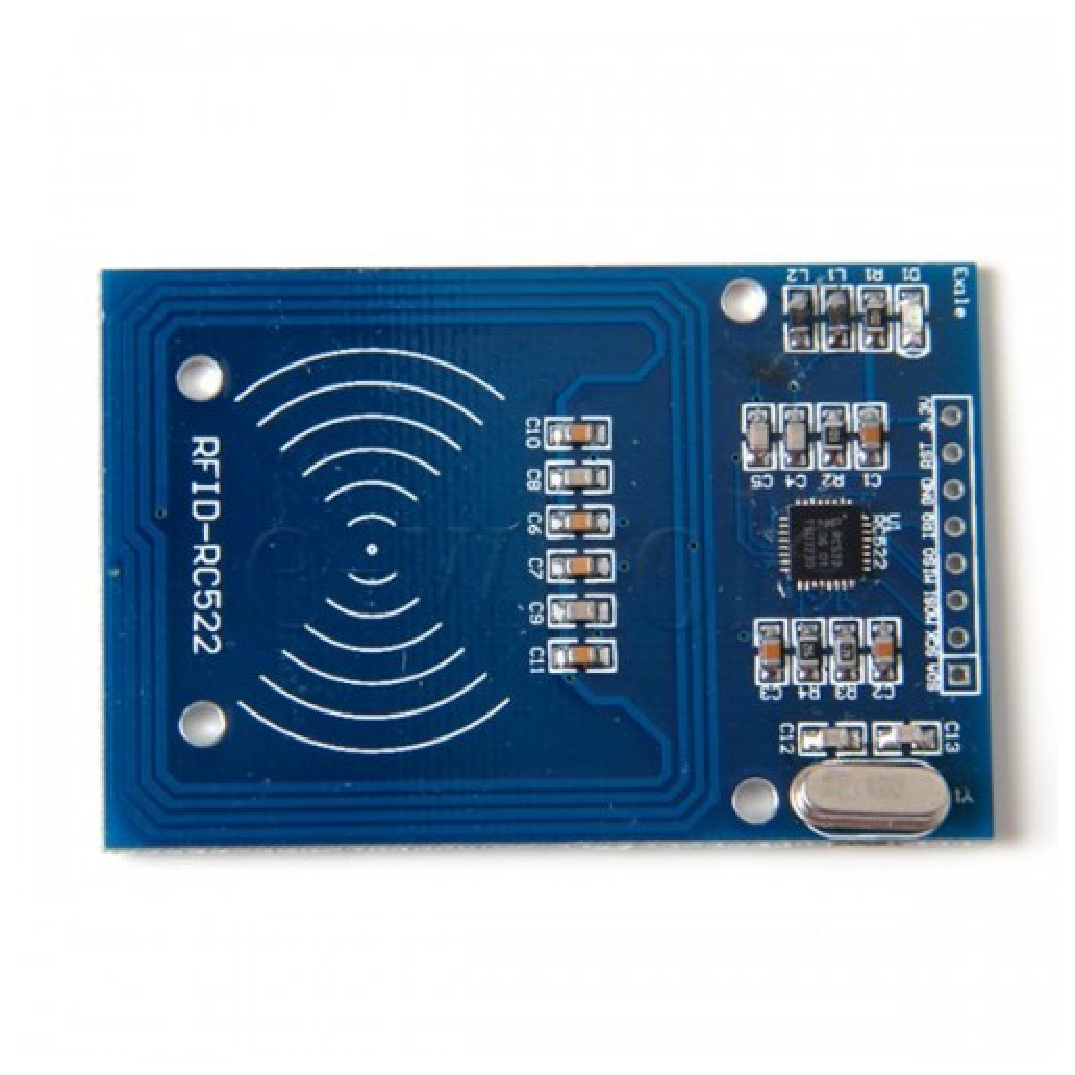
\includegraphics[keepaspectratio=true,scale=0.5]{figuras/rfid.eps}
  \caption{Módulo Leitor Rfid Mfrc522 Mifare}
\end{figure}


\subsection{Módulo WiFi ESP8266 ESP-01}
O módulo wireless ESP8266 foi desenvolvido para que seja possível conectar o microcontrolador a uma conexão WiFi de forma fácil, eficaz e a um baixo preço.

Este módulo suporta as redes 802.11 b/g/n, muito usadas atualmente, podendo trabalhar como um Ponto de Acesso (Access Point) ou como uma Estação (Station), enviando e recebendo dados.

A comunicação serial pelo protocolo RS-232, irá utilizar as portas RX(pino 45) e TX(pino 46) do microcontrolador que possuem suporte para este protocolo de comunicação TX e diretamente a protoboard. Ele será utilizado para enviar as informações coletadas pelo dispositivo ao banco de dados na rede.
\pagebreak

\begin{figure}[!ht]
  \centering
  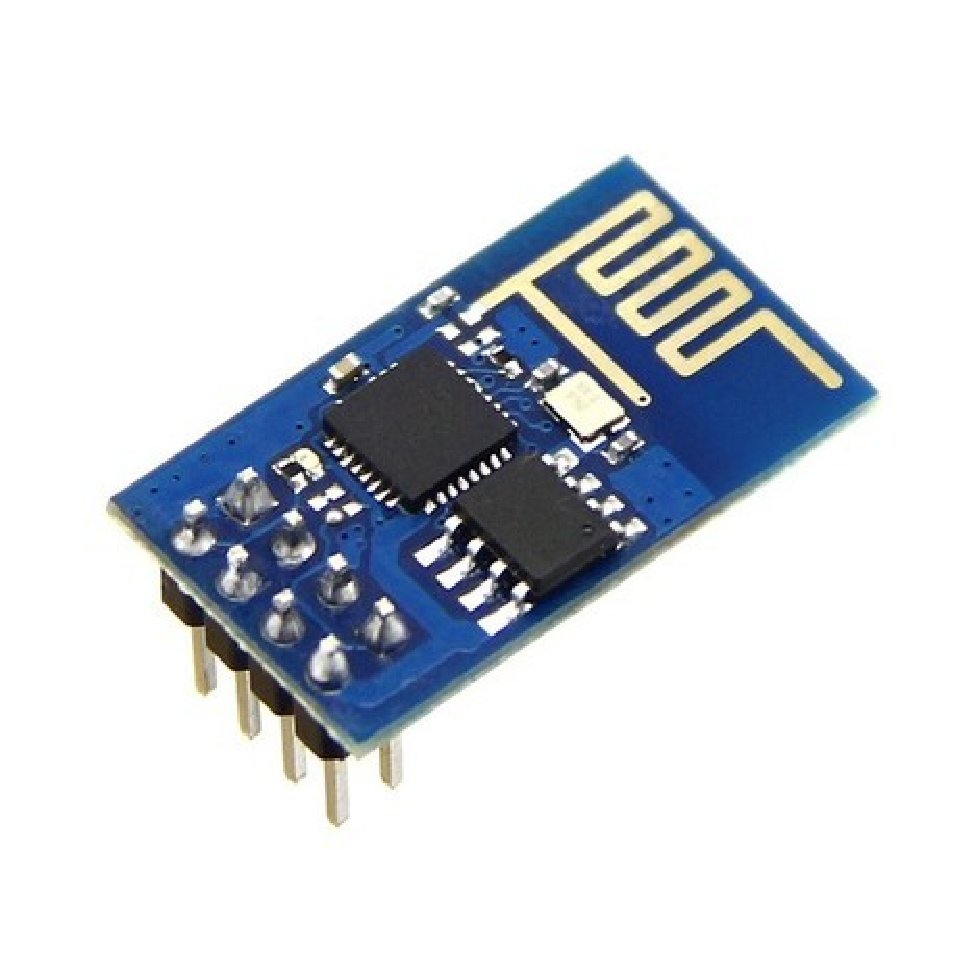
\includegraphics[keepaspectratio=true,scale=0.5]{figuras/wifi.eps}
  \caption{Módulo Leitor Rfid Mfrc522 Mifare}
\end{figure}


\subsection{Display LCD 16x2}
Este é um display LCD de 16 colunas por 2 linhas, backlight azul e escrita branca. Possui o controlador HD44780 usado em toda indústria de LCD's como base de interface.

A interface com microcontrolador é muito simples, sendo basicamente 4 pinos digitais de dados e 2 pinos digitais de controle. Confira no link o Datasheet Display LCD 16x2. O display será utilizado para mostrar a matrícula e o nome do dono da carteirinha, possibilitar ao professor selecionar a disciplina que deseja passar a chamada e outras informações que forem necessárias.

\begin{figure}[!ht]
  \centering
  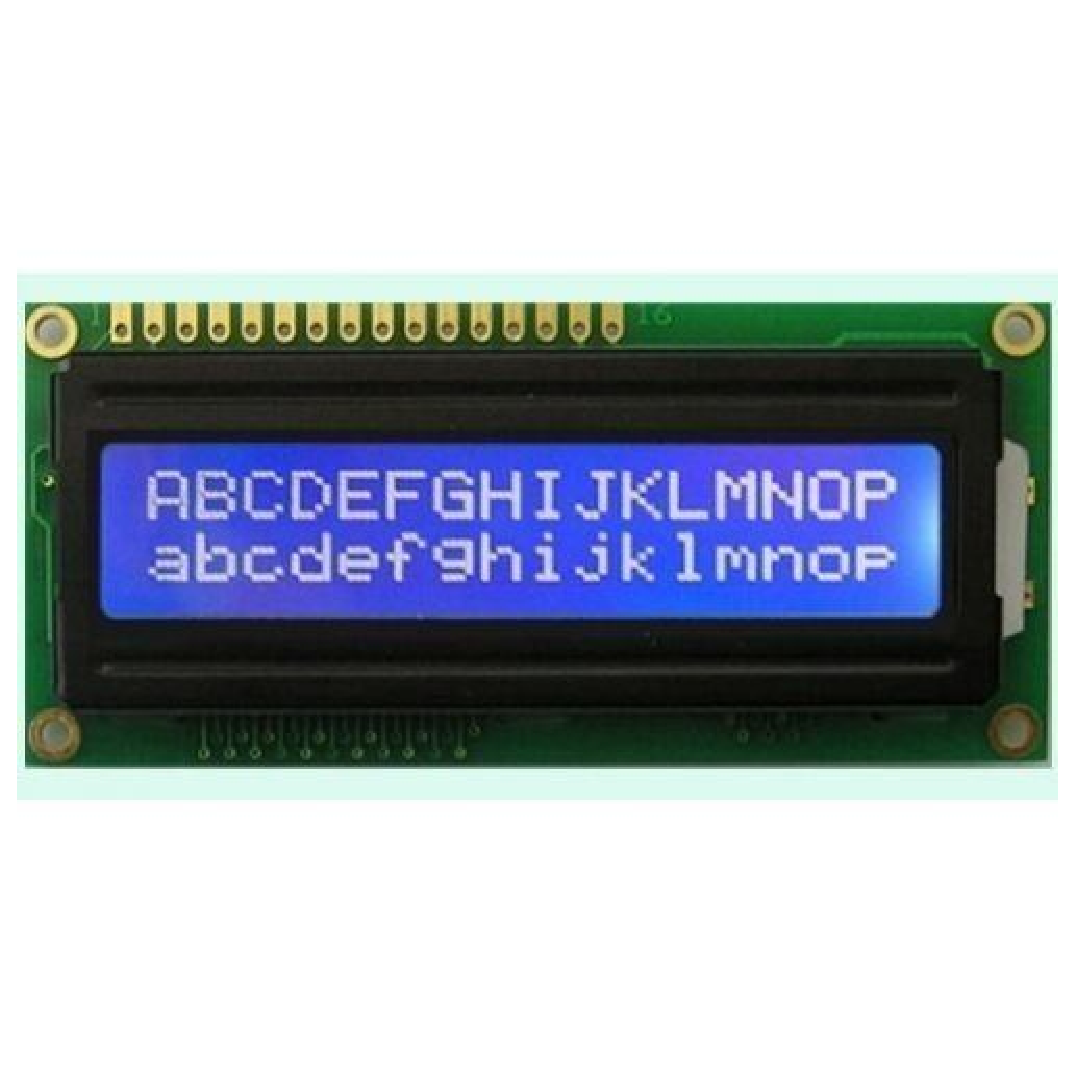
\includegraphics[keepaspectratio=true,scale=0.45]{figuras/lcd.eps}
  \caption{Display LCD}
\end{figure}

\pagebreak

\subsection{Teclado de Película 4x4}
O Teclado Matricial 4x4 é um componente utilizado para entrada de dados. Ele possui 16 teclas dispostas em 4 linhas x 4 colunas, e um conector de 8 pinos para ligação. Ele necessita de 8 pinos digitais para funcionar, sendo 4 configurados como saída(OUTPUT) e 4 como leitura(INPUT). Os pinos de saída são acionados como um contador em anel, elevando um pinos em nível alto e os demais em nível baixo, após um tempo determinado outro pino fica em nível alto e o resto em nível baixo e o ciclo se repete para cada pino. Cada pino é conectado em uma coluna da matriz e os pinos de leitura lêem as quatro linhas individualmente. Desta forma quando um botão é pressionado,  é possível determinar a linha e coluna da matriz.

\begin{figure}[!ht]
  \centering
  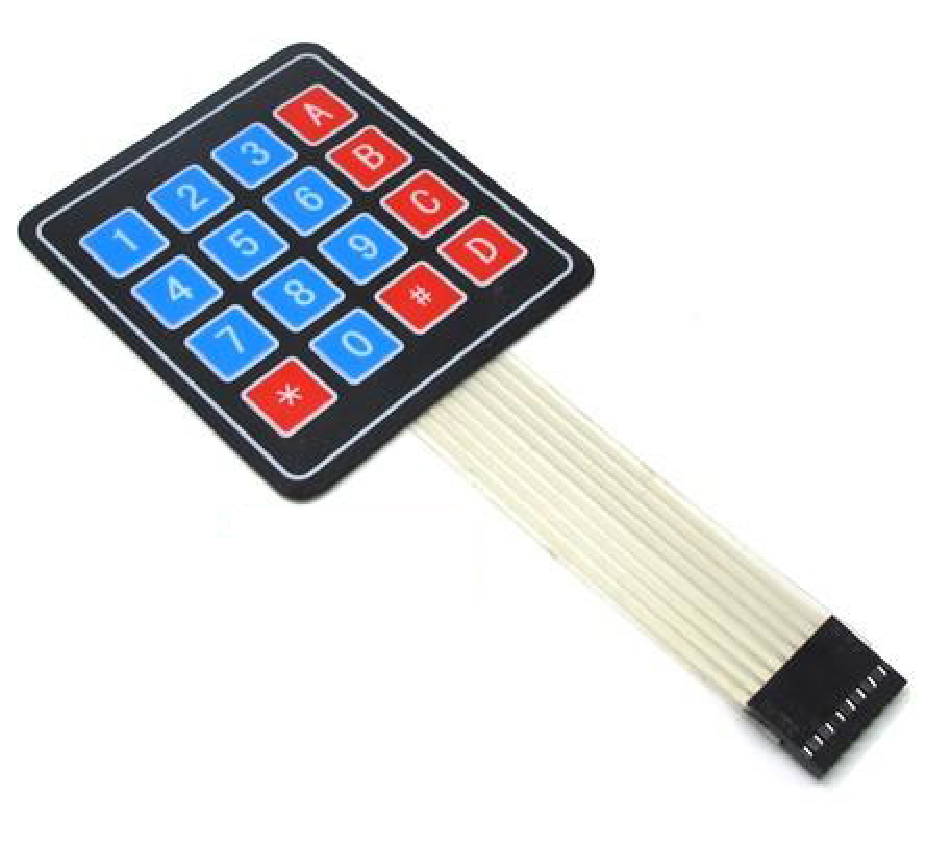
\includegraphics[keepaspectratio=true,scale=0.45]{figuras/teclado.eps}
  \caption{Teclado de Película 4x4}
\end{figure}

\subsection{Carregador de Bateria Lipo - Mini Usb TP4056}
Módulo carregador de baterias TP4056 para baterias de lítio, possibilita que as baterias sejam recarregadas sem a necessidade de removê-las do circuito. Módulo se conecta diretamente com a bateria e carrega a mesma quando é conectado um carregador USB. A corrente é cortada quando detecta que a carga está completa e possui um led indicador de carregamento. Contudo para aferir o nível de carga da bateria, será utilizado um pino analógico do microcontrolador. Medindo o nível de tensão na bateria será possível  informar o  nível de  carga através do display LCD, o que é mais prático.


\begin{figure}[!ht]
  \centering
  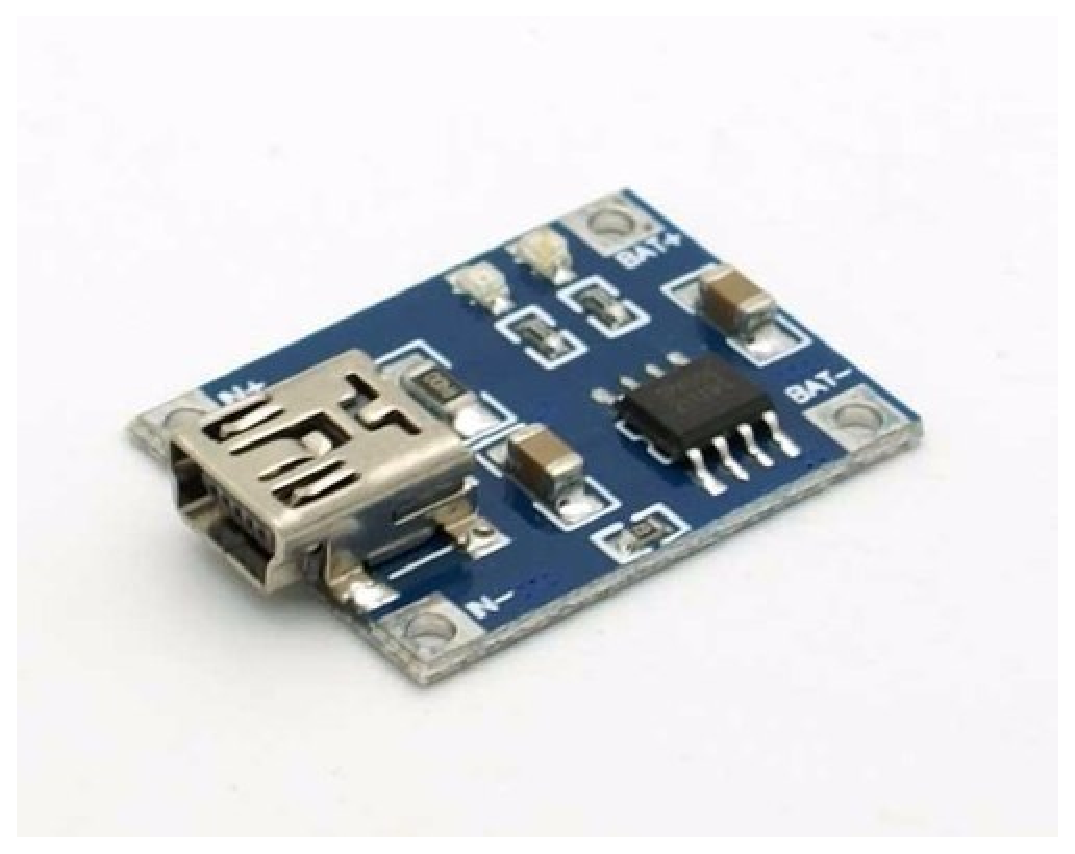
\includegraphics[keepaspectratio=true,scale=0.45]{figuras/carregador.eps}
  \caption{Carregador de Bateria Lipo}
\end{figure}

\subsection{Bateria}
Serão utilizadas duas baterias 3.7V 2000mAh em série para alimentar o dispositivo. A tensão fornecida será 7.4~6V e uma autonomia de cerca de 8 horas em uso á 157 horas (cerca de 6 dias) em \textit{standby}. Todos os componentes têm uma tensão de operação de 3.3V, apenas o display LCD opera com 5V. Para regular a tensão, será utilizado CI regulador de tensão 7805 para o display e o LM1117T para os demais.

\begin{figure}[!ht]
  \centering
  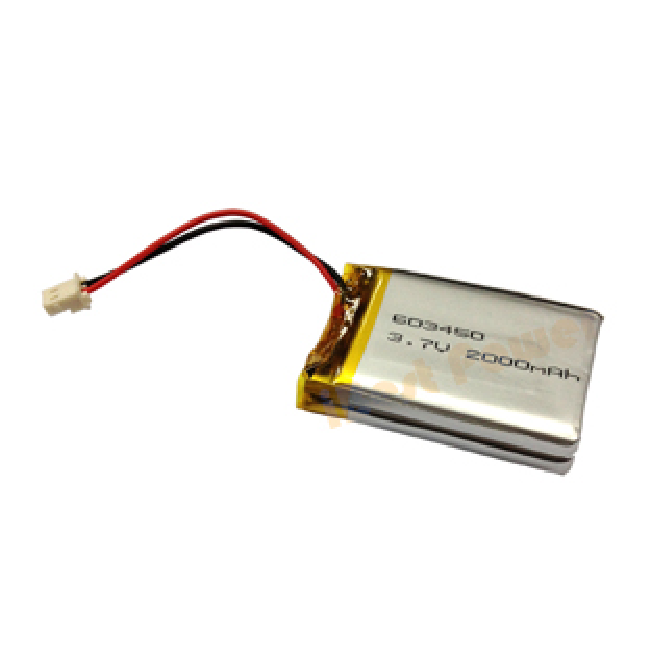
\includegraphics[keepaspectratio=true,scale=0.7]{figuras/bateria.eps}
  \caption{Bateria 2000mAh}
\end{figure}

\subsection{Microcontrolador ATmega1280}
O microcontrolador escolhido foi o ATmega1280 em função de ser o microcontrolador presente no Arduino Mega e seu número de pinos. Por isso, será possível utilizar o bootloader do arduino no microcontrolador, facilitando a programação uma vez que todos os componentes utilizados no projeto possuem bibliotecas que facilitam seu uso e implementação para arduino. Seu número de pinos digitais e especiais (TX, RX, MOSI, MISO, SDA, SCK) também foi levado em consideração durante o processo de escolha.

Em seguida, foram testados e pesquisados dados de tensão, autonomia e corrente, devido ser um aparelho portátil e de funcionamento independente da internet e sem estar ligado na tomada. Todos os dados estão apresentados na tabela a seguir.

\begin{table}[!ht]
  \centering
  \caption{Dados dos Componentes - Aparelho de Frequência}
  \begin{tabular}{|l|c|c|c|}
    \hline
    \multicolumn{1}{|c|}{\textbf{Componentes}}                  & \parbox[t]{2cm}{\textbf{Corrente máxima (mA)}} & \multicolumn{1}{l|}{\parbox[t]{2cm}{\textbf{Corrente mínima (mA)}}} & \parbox[t]{5cm}{\textbf{Tensão de nominal (V)}} \\ \hline
    \parbox[t]{6cm}{Kit Módulo Leitor Rfid Mfrc522 Mifare\\}                       & 13                            & 10                                        & 3,3                            \\ \hline
    \parbox[t]{6cm}{Cartão RFID Programável Mifare 13,56Mhz}                     & -                             & -                                         & -                              \\ \hline
    Módulo WiFi ESP8266 ESP-01                                  & 215                           & 0,9                                       & 3,3                            \\ \hline
    LCD 16x2                                                    & 1,5                           & 1                                         & 5                              \\ \hline
    Teclado de película 4x3                                     & 0,3                           & 0,3                                       & 3,3                            \\ \hline
    ATmega1280                                                  & 20                            & 0,5                                       & 1,8                     \\ \hline
    \parbox[t]{6cm}{Carregador De Bateria   Lipo - Mini Usb Tp4056}                & 0                             & 0                                         & 5                              \\ \hline
    Bateria 3,7v 2000mah                                        & 0                             & 0                                         & 3,7                            \\ \hline
    \multicolumn{1}{|c|}{\textbf{TOTAL}}                        & 249,8                         & 12,7                                      & -                              \\ \hline
  \multicolumn{1}{|c|}{\parbox[t]{5cm}{\textbf{Autonomia da bateria (Horas)}}} & 8                             & 157                                       & -                              \\ \hline
  \end{tabular}
\end{table}

Com base nos dados da tabela anterior, pode-se afirmar que a autonomia da bateria do dispositivo em uso contínuo poderá ser de até 8 horas e, em standby, até 6 dias. Dado que o dispositivo poderá entrar em um modo de dormência, desabilitando o wifi, o leitor e até o próprio microcontrolador, ele poderá ter uma autonomia maior que 8 horas se entrar de forma automática neste modo enquanto aguarda uso.

Por fim, em termos econômicos, obtivemos o seguintes dados de custos:

\begin{table}[!ht]
  \centering
  \caption{Custos dos Componentes - Aparelho de Frequência}
  \label{my-label}
    \begin{tabular}{|l|c|c|}
    \hline
    \multicolumn{1}{|c|}{\textbf{Componente}}    & \textbf{Custo} & \textbf{Fonte}                                                                                                \\ \hline
    \parbox[t]{7cm}{Kit Módulo Leitor Rfid Mfrc522 Mifare}        & R\$ 39,90      & \href{http://www.filipeflop.com/pd-6b883-kit-modulo-leitor-rfid-mfrc522-mifare.html}{Fonte 1}                                 \\ \hline
    \parbox[t]{7cm}{Cartão RFID Programável Mifare 13,56Mhz}      & R\$ 5,90       & \href{http://www.filipeflop.com/pd-1c240a-cartao-rfid-programavel-mifare-13-56mhz.html}{Fonte 2}                              \\ \hline
    Módulo WiFi ESP8266 ESP-01                   & R\$ 29,90      & \href{http://www.filipeflop.com/pd-1f55ad-modulo-wifi-esp8266-esp-01.html}{Fonte 3}                                           \\ \hline
    LCD 16x2                                     & R\$ 16,90      & \href{http://www.filipeflop.com/pd-6b7e4-display-lcd-16x2.html?ct=\&p=1\&s=1}{Fonte 4}                                        \\ \hline
    Teclado de película 4x3                      & R\$ 10,90      & \href{http://www.filipeflop.com/pd-218a98-teclado-matricial-de-membrana-12-teclas.html?ct=\&p=1\&s=1}{Fonte 5}                \\ \hline
    ATmega1280                                   & R\$ 60,00      & \href{http://produto.mercadolivre.com.br/MLB-831270785-lote-5-pecas-atmega1280-16au-marca-atmel-100-tqfp-atmel-\_JM}{Fonte 6} \\ \hline
    \parbox[t]{7cm}{Carregador De Bateria Lipo - Mini Usb Tp4056} & R\$ 9,90       & \href{http://www.filipeflop.com/pd-36ef09-modulo-carregador-de-baterias-de-litio-tp4056.html?ct=\&p=1\&s=1}{Fonte 7}          \\ \hline
    Bateria 3,7v 2000mah                         & R\$ 19,90      & \href{http://produto.mercadolivre.com.br/MLB-763262237-bateria-tablet-universal-dl-navcity-phaser-37v-2000mah-\_JM}{Fonte 8}  \\ \hline
\end{tabular}
\end{table}

Apesar da tabela não apresentar os preços do case superior e inferior, todo o aparelho ficaria em torno de R\$ 193,30. Este é um preço considerado acessível, considerando o tempo que o aparelho pode manter um bom funcionamento.

\section{Acesso às Salas e Laboratórios}
O controle de acesso às salas e laboratórios será um sistema único na faculdade, porém alunos e professores terão um tratamento diferenciado para a liberação de entrada nas salas. Essa diferenciação ocorre principalmente pelo fato dos ambientes possuírem equipamentos caros e pela segurança dos alunos e professores durante as aulas.

\subsection{Acesso dos Professores}
Para obterem acesso às salas, os professores terão que apresentar seu cartão no leitor RFID, que por sua vez lerá
 os arquivos guardados no chip, matrícula e nome completo do docente, e gerará o token de segurança. Assim que esses
  dados de entradas forem lidos pelo aparelho, o módulo wifi do equipamento se conectará imediatamente com a rede da
   faculdade e vai comparar os dados de entrada com os que estão no banco de dados já salvos pela UnB, e caso os
    dados estejam de acordo, a placa controladora do aparelho fará conexão com os outros micro equipamentos e a
     tranca será liberada para o acesso a sala ou laboratório. Enquanto o professor não passar novamente o cartão
      para fechar a sala, a porta ficará destrancada para a entrada dos alunos.

Caso o professor esqueça o cartão seria possível a entrada nas salas por meio de uma senha cadastrada, sendo que
 essa senha somente os professores terão acesso, e cada um dos professores terá sua senha própria. Vale ressaltar
  que o horário em que o professor inicia a abertura da sala, sempre é registrado, assim como o horário de fechamento.
   Os professores terão permissão para fazer o uso de qualquer sala ou laboratório em qualquer horário em que a universidade esteja aberta.

\subsection{Acesso dos Alunos}
Para um aluno abrir as salas com trancas será necessário que ele apresente sua carteirinha com nome e matrícula na secretaria, e lá ele receberá uma senha provisória. Isso se deve ao fato de que quando um aluno passar a carteirinha no leitor RFID e o leitor fizer todo seu processo de reconhecimento, o dispositivo reconhecerá que é um aluno tentando entrar e será solicitada uma senha para ele ter o acesso nas salas. Neste caso, o dispositivo vai registrar o horário e o tempo de uso da sala no qual o aluno se responsabilizará durante esse tempo.

Caso o aluno responsável pela sala tenha que sair, será necessário que outro aluno faça o mesmo procedimento para que a sala continue aberta, fazendo com que a responsabilidade também mude para o novo aluno cadastrado. No caso das salas de estudos, em que não terão controle de acesso, todos terão entrada livre para maior liberdade de acesso dos alunos, inclusive daqueles que não são alunos da universidade.

Para a escolha do sistema RFID no controle das salas, foi feito um balanço financeiro sobre possíveis possibilidades de marcas e compradores diferentes, como é mostrado na tabelas a seguir.

\begin{table}[h]
  \centering
  \caption{Custos - Dispositivo de Frequência}
  \begin{tabular}{l|l|}
    \cline{2-2}
    \textbf{Preço Unitário}   & \multicolumn{1}{c|}{R\$ 193,30} \\ \cline{2-2}
    \textbf{TOTAL (20 salas)} & R\$ 3.866,00                    \\ \cline{2-2}
  \end{tabular}
\end{table}

\begin{table}[h]
  \centering
  \caption{Custos - Fechaduras}
  \label{my-label}
  \begin{tabular}{|l|l|c|l|c|l|}
    \hline
    \multicolumn{2}{|c|}{\parbox[t]{3cm}{\textbf{INTELBRAS FFX 1000}}} & \multicolumn{2}{c|}{\textbf{C90 HDL}}       & \multicolumn{2}{c|}{\parbox[t]{3cm}{\textbf{PROTECTION PT-710}}} \\ \hline
    \textbf{Loja}                 & \textbf{Preço}    & \textbf{Loja}              & \textbf{Preço} & \textbf{Loja}                & \textbf{Preço}   \\ \hline
    \parbox[t]{2cm}{MAGAZINE LUIZA}                & R\$ 143,91        & AMERICANAS                 & R\$ 165,90     & \parbox[t]{2cm}{PROTECTION STORE}             & R\$ 219,00       \\ \hline
    WALMART                       & R\$ 145,00        & WALMART                    & R\$ 169,00     & WALMART                      & R\$ 131,00       \\ \hline
    MERCADO LIVRE                 & R\$ 145,90        & \parbox[t]{2cm}{MERCADO LIVRE}              & R\$ 149,90     & \parbox[t]{2cm}{MERCADO LIVRE}                & R\$ 125,00       \\ \hline
    SUBMARINO                     & R\$ 145,90        & SUBMARINO                  & R\$ 179,90     & -                            & -                \\ \hline
    \parbox[t]{2cm}{RICARDO ELETRO}                 & R\$ 180,40        & \parbox[t]{2cm}{LEROY MERLIN}               & R\$ 179,90     & -                            & -                \\ \hline
    \textbf{MÉDIA:}               & R\$ 152,22        & \textbf{MÉDIA:}            & R\$ 168,92     & \textbf{MÉDIA:}              & R\$ 168,92       \\ \hline
    \parbox[t]{2cm}{\textbf{TOTAL (20 SALAS):}}    & R\$ 3.044,44      & \parbox[t]{2cm}{\textbf{TOTAL (20 SALAS):}} & R\$ 3.378,40   & \parbox[t]{2cm}{\textbf{TOTAL (20 SALAS):}}   & R\$ 3.166,67     \\ \hline
  \end{tabular}
\end{table}

A primeira tabela se refere ao dispositivo utilizado que é o mesmo do controle de frequência, já mencionado anteriormente com mais detalhes. A segunda tabela, por sua vez, mostra um detalhamento sobre os tipos de fechadura visto por empresas diferentes. Analisando toda a tabela, é notável que a fechadura Intelbras FFX 1000 tem um preço mais acessível, comparado às outras, além de ser tão eficiente quanto todas pesquisadas.

\section{Acesso ao Estacionamento}

Já foram apresentadas anteriormente (no Ponto de Controle 1) as vantagens e desvantagens do controle do acesso ao estacionamento. Em resumo: por um lado temos a sonhada segurança no campus da FGA e por outro lado temos a rejeição do público alvo com o novo sistema.

O sistema funcionará utilizando um leitor RFID de baixa frequência, essa gama de frequências estende-se dos 30KHz aos 300KHz. Os leitores, nesta gama de frequências, operam a 125 ou 135 KHz e possuem um alcance inferior a meio metro com a velocidade de transferência inferior a 1 kbits/s, o que significa que este opera em baixa interferência com o meio ambiente e tem um comportamento bom na leitura de tags em objetos contendo líquidos e metais, assim todo o processo do microcontrolador de chegar no banco de dados as informações do aluno, professor ou funcionário acontecerá, e permitirá ou não a passagem do carro para o estacionamento privativo.

Além de contar com o aparelho leitor RFID e a cancela para controlar o acesso, o estacionamento também terá uma câmera que filmará em tempo real a placa do carro e o motorista, constatando o horário de saída e entrada do carro.

Apesar desse sistema de segurança ser primordial no projeto, ele é um sistema de fácil implementação e uso, tendo em vista que não há um diferenciamento específico de pessoas que entram no estacionamento. Qualquer pessoa da faculdade pode entrar sem exceções e o sistema de banco de dados com nome e matrícula é o mesmo que outras partes de controle de acesso também utilizam.

Em termos financeiros, o projeto de controle de acesso ao estacionamento é considerado viável devido ao \textit{payback} de todos os equipamentos utilizados com é mostrado na tabela a seguir.

\pagebreak

\begin{table}[h]
  \centering
  \caption{Custos - Estacionamento}
  \begin{tabular}{|l|l|l|l|l|l|l|}
    \hline
    \multicolumn{2}{|c|}{\textbf{Item}} & \multicolumn{2}{c|}{\textbf{Quantidade}} & \multicolumn{1}{c|}{\textbf{Descrição}}                                                               & \textbf{R\$ (unidade)} & \textbf{R\$ (total)} \\ \hline
    \multicolumn{2}{|l|}{1}             & \multicolumn{2}{l|}{2}                   & \parbox[t]{6cm}{Instalação de CPU ou totens de leitura de tags RFID.}                                                  & R\$678,00              & R\$1.356,00          \\ \hline
    \multicolumn{2}{|l|}{2}             & \multicolumn{2}{l|}{2}                   & Hardware de comunicação com cancelas.                                                                 & R\$800,00              & R\$1.600,00          \\ \hline
    \multicolumn{2}{|l|}{3}             & \multicolumn{2}{l|}{2}                   & \parbox[t]{6cm}{Sensores de leitura infra-vermelho, para identificação da saida de veiculos e fechamento de cancelas.} & R\$1.200,00            & R\$2.400,00          \\ \hline
    \multicolumn{6}{|l|}{\textbf{TOTAL:}}                                                                                                                                                                           & R\$5.356,00          \\ \hline
  \end{tabular}
\end{table}

Apesar de serem equipamentos caros, estes possuem uma longa vida útil, se usados corretamente, ou seja, se trata de um investimento à longo prazo de um bem útil à todo o corpo universitário.



Vale a pena ressaltar que o aparelho de frequência é o mesmo utilizado em todas as frentes de controle de acesso, a única diferença entres as frentes é que para o controle nas salas e controle do estacionamento ele estará preso em uma superfície plana na vertical, para que o usuário possa fazer uso dele tanto em pé quanto dentro do automóvel.







\chapter[Instrumentação e Controle]{Instrumentação e Controle}

\section{Ambientação da Sala}
\subsection{Iluminação}

Nas salas de aula serão utilizadas um modelo de lâmpada inteligente que possui sensores de luminosidade e de presença. Este equipamento é capaz de ajustar a intensidade luminosa do ambiente, permitindo a manutenção automática do nível adequado de luz. A curto prazo, essa solução se apresenta um custo elevado, pois cada kit (2 lâmpadas e 1 controlador) custa cerca de R\$ 500,00. Porém, a longo prazo, possui maior custo benefício, pois apresentam uma vida útil de aproximadamente 30 anos. A lâmpada chega a consumir 60\% a 80\% (de 598,4 W/H a  1196,8 W/H) do consumo de energia elétrica comparada a uma lâmpada LED tradicional (cerca de 2992 W/H).

\subsection{Persianas Inteligentes}

Persianas automatizadas serão utilizadas para o controle de iluminação natural nos ambientes do prédio. Estas persianas são feitas de um material resistente, e podem serão instaladas na parte interna das salas. O espaçamento entre cada haste pode ser regulado, para limitar a quantidade de luz natural que entra na sala. Além disso, a fabricação das persianas impede a entrada de poeira, reduzindo os problemas que ela causa, e quando totalmente fechadas, fornecem isolamento acústico.
As persianas são controladas a partir de um mesmo ponto, simplificando e diminuindo a movimentação para abrí-las ou fechá-las dentro da sala. Seu custo médio é de R\$ 450,00.

\subsection{Sistema de Som}

Para a sonorização do ambiente da sala de aula, serão utilizadas caixas de som in-wall, com potência máxima de 160 Watts e armação reforçada de fibra de vidro. O custo é de aproximadamente R\$570,00 o par.
Para os microfones, serão utilizados dispositivos sem fio e com apoio na orelha, comodidade para o professor. O preço varia bastante, sendo encontrados valores por volta de R\$ 150,00.

\subsection{Climatização}

Serão utilizados ar-condicionados do tipo split inverter, o qual o compressor nunca desliga, então não ocorre picos de energia. Além disso, esse compressor tem a velocidade de rotação variável, se auto-regulando de acordo com a temperatura interior. Apresentam um maior custo, porém, economizam energia ao longo do tempo, o que traz benefícios.
Para as salas de aula menores, serão utilizados aparelhos com 12.000 BTUs de potência, que custa em torno de R\$1.200,00. Pela tabela do Procel o ar-condicionado de 12.000 BTUs split consume aproximadamente 193,76 KW/h.
Para as salas maiores, serão utilizados ar-condicionados mais potentes, devido a grande quantidade de alunos nas aulas e o tamanho das salas. Estes equipamentos terão 58000 BTUs de potência, que custam R\$5000,00 e pela tabela de do Procel ele consome cerca de 679,20 KW/h de energia elétrica.

\begin{table}[!ht]
  \centering
  \caption{Soluções de Ambientação da Sala}
  \label{my-label}
    \begin{tabular}{|l|l|l|l|l|l|}
    \hline
    \textbf{Equipamentos} & \textbf{Descrição} & \textbf{Vantagens} & \textbf{Desvantagens} & \textbf{Consumo} & \textbf{Custo} \\ \hline
    \parbox[t]{3cm}{Lâmpada Inteligente} & \parbox[t]{2cm}{Lâmpada inteligente que possui sensores de luminosidade e de presença.} & \parbox[t]{3cm}{Economia de energia, longa durabilidade e sensores de nível de luz.} & \parbox[t]{3cm}{Custo comparado com as outras lâmpadas.} & \parbox[t]{2cm}{Entre 1196,8W/H e 598,4WH.} & \parbox[t]{2cm}{R\$560,00} \\ \hline
    \parbox[t]{3cm}{Persianas Automatizadas} & \parbox[t]{2cm}{Persianas automatizadas que funciona a partir de um determinado aplicativo.} & \parbox[t]{3cm}{Facilidade na hora de escolher abertura da persiana.} & \begin{tabular}[c]{@{}l@{}}\parbox[t]{3cm}{Falta de energia do prédio compromete o funcionamento}\\ \parbox[t]{3cm}{Custo comparado com uma persiana normal.}\end{tabular} & \parbox[t]{2cm}{Não foi encontrado.} & \parbox[t]{2cm}{R\$450,00} \\ \hline
    \parbox[t]{3cm}{Alto-Falantes} & \parbox[t]{2cm}{Caixas de som que são fixadas na parede.} & \parbox[t]{3cm}{Melhor propagação do som pela sala.} & \parbox[t]{3cm}{Falta de energia compromete o uso, e se tiver problemas de funcionamento compromete o som da sala.} & \parbox[t]{2cm}{160 Watts.} & \parbox[t]{2cm}{R\$570,00 o par.} \\ \hline
    \parbox[t]{3cm}{Microfones} & \parbox[t]{2cm}{Aparelho que converte ondas sonoras em sinais elétricos.} & \parbox[t]{3cm}{Aumento da voz do professor e melhora a qualidade de som das aulas.} & \parbox[t]{3cm}{Falta de energia compromete o uso e se tiver problemas de funcionamento pode prejudicar a qualidade do som durante as aulas.} & \parbox[t]{2cm}{12 Watts.} & \parbox[t]{2cm}{R\$ 150,00} \\ \hline
    \parbox[t]{3cm}{Ar-condicionado} & \parbox[t]{2cm}{Aparelho que regula o aquecimento ou a refrigeração do ambiente.} & \parbox[t]{3cm}{Monitoramento da temperatura do ambiente e melhora o clima da sala principalmente em épocas de calor.} & \parbox[t]{3cm}{Custo e alto gasto de energia ainda mais nas salas grandes.} & \parbox[t]{2cm}{193,76 KW/h a 679,20KW/h} & \parbox[t]{2cm}{R\$1.298,0 a R\$5449,00} \\ \hline
  \end{tabular}
\end{table}

\section{Digitalização e Integração de Equipamentos para Aula}

\subsection{Mesa Inteligente}

A mesa inteligente consiste em uma tela sensível ao toque, em formato de mesa, que permitirá que o professor controle os diversos dispositivos presentes na sala.
As características de cada dispositivo varia de um fabricante para outro, como por exemplo o tamanho da tela sensível ao toque, sendo encontradas usualmente telas de 32 a 65 polegadas, ou a presença de tecnologias de reconhecimento de objetos colocados sobre sua superfície.
As mesas interativas possuem suporte para diferentes sistemas operacionais, como Windows, Linux, MacOs X, e até Android, o que permite a fácil integração com outros dispositivos como projetores e roteadores de internet. Isto pode possibilitar ao professor o acesso a materiais disponíveis online durante a aula, facilidade de exibição de apresentações em slides entre outras inúmeras possibilidades de uso, além de possuir um controle centralizado de todas as funções automatizadas presentes na sala de aula.

\subsection{Quadro interativo}

Além dos quadros convencionais, um quadro interativo será utilizado para auxiliar o professor, tornando as aulas expositivas mais dinâmicas. Atualmente existem diversos fabricantes de quadros interativos, com diferentes tamanhos e funcionalidades, incluindo até, em alguns casos, suites de softwares específicos para aquele determinado produto. Os dispositivos possuem diversas opções de conectividade, possibilitando a interação com computadores pessoais, dispositivos mobile e até mesmo com a mesa inteligente do professor. O custo deste equipamento varia entre R\$4.000,00 e R\$8.000,00.

\begin{table}[!ht]
  \centering
  \caption{Soluções de Digitalização e Integração de Equipamentos para Aula}
  \label{my-label}
  \begin{tabular}{|l|l|l|l|l|l|}
    \hline
    \textbf{Equipamentos} & \textbf{Descrição} & \textbf{Vantagens} & \textbf{Desvantagens} & \textbf{Consumo} & \textbf{Custo} \\ \hline
    \parbox[t]{3cm}{Mesa inteligente} & \parbox[t]{2cm}{Painel de controle da sala e também um computador de uso do professor}. & \parbox[t]{3cm}{Auxilia no monitoramento do professor em relação a sala e além de ser um instrumento a mais de uso para as aulas dos professores e na aprendizagem dos alunos.} & \parbox[t]{3cm}{Alto custo e se for danificado pode comprometer as aulas dos professores e do funcionamento da sala.} & \parbox[t]{2cm}{Não encontrado.} & \parbox[t]{2cm}{\$8000,00 (Dólares)} \\ \hline
    \parbox[t]{3cm}{Quadro interativo} & \parbox[t]{2cm}{Superfície que,reconhece a escrita electronicamente e que necessita de um computador para funcionar.} & \parbox[t]{3cm}{Aumento na produtividade e exposição do conteúdo das aulas e além de ser mais uma ferramenta útil para os professores.} & \parbox[t]{3cm}{Alto custo e restrito ao local.} & \parbox[t]{2cm}{0,5W} & \parbox[t]{2cm}{Entre R\$4.000,00 e R\$8.000,00} \\ \hline
  \end{tabular}
\end{table}

\section{Status da Sala}

\subsection{Painel informativo}

A melhor solução para o painel informativo seria um display de LCD embutido na parede, onde as informações sobre o status da sala serão exibidas. Estas informações seriam enviadas em tempo real, permitindo que imprevistos ou informações de última hora sejam informadas aos usuários da sala com maior efetividade. O custo deste tipo de equipamento varia em torno de R\$300,00 e R\$1500,00, dependendo da marca e do tamanho da tela.

\section{Sensores}

\subsection{Termopar}

Os termopares medem a temperatura do ambiente utilizando-se de dois condutores metálicos diferentes unidos na mesma extremidade. Esse dispositivo funciona pelo princípio de que essa configuração citada, gera uma força eletromotriz em função dos metais e das temperaturas T1 (junta de medida) e T2 (junta de referência). Assim criou-se uma tabela de correlação entre a FEM e a função de temperatura, considerando T2=0. Para o nosso projeto, foi escolhido o termopar tipo K que é de uso genérico, tem baixo custo e mede temperaturas entre -200 e 1200C, tendo uma sensibilidade de aproximadamente 41uV/C. O custo de um termopar é de aproximadamente R\$40,00.

\subsection{Termostato}

É o dispositivo utilizado para manter a temperatura constante, composto por um sensor que mostra a variação de temperatura e um que controla essa variação. Aqui pode se aplicar o Ecobee 3 que custa \$169. Esse aparelho possui um sensor de movimento, priorizando sua utilização onde detecta movimento e ainda mantém a tela em modo de economia de energia até detectar que alguém está se aproximando da tela. Ele funciona via Wi-fi e aplicativos, além do que pode se conectar a mesa inteligente.

\subsection{Sensores de Calor}

Será usado como sensor de calor o detector de temperatura e Fumaça Combinados, código AFVRFTH da empresa ABAFIRE. É um equipamento que deve ser instalado no teto ou na parede das edificações e tem como função enviar um alerta para uma Central de Alarme de Incêndio assim que detecta o aumento brusco da temperatura ambiente ou a presença de fumaça. Este alerta serve para avisar ao responsável pela segurança da edificação que, possivelmente, existe uma situação emergencial no local, como um princípio de incêndio . O sensor consegue identificar pela elevação da temperatura quanto pela presença de fumaça.Ele detecta a partir dos 55C e tem uma cobertura circular de 4,2 metros. É alimentado com 24V .Possui LED vermelhos de vigília e alarme.Consumo de 30 uA em repouso e 30MA quando é ativado. O sensor estaria interligado com a sala de controle para que seja avisado o perigo de incêndio no local e ele se encontra no mercado entre R\$150 e R\$ 250.

\subsection{Sensor de movimento}

O sensor de movimento será utilizado para o controle de luz do ambiente, fazendo com que não tenha desperdício de energia ao deixar as luzes ligadas. Esse sensor seria basicamente para, no caso de deixarem a luz ligada, depois de um certo tempo e verificando que não tem ninguém no local, as luzes sejam apagadas automaticamente. O preço dos sensores varia, tendo sensores que custam R\$15,00 (no caso, seria apenas o sensor, tendo que fazer o circuito para o funcionamento do mesmo) e sensores prontos para uso, que variam o preço entre R\$35,00 e R\$ 210,00.

\subsection{Fototransistores}

Dispositivo utilizado na lâmpada responsiva, que variam a resistência elétrica de acordo com a intensidade luminosa do local. Ele possui dois diodos de junção, o coletor e o emissor; a base é incluída quando tem-se polarização ou controle elétrico. Quando recebem fótons, o conjunto base-coletor cria lacunas na sua vizinhança e a tensão faz com que as lacunas sejam transmitidas para o emissor. Enquanto isso os elétrons do emissor sao tranferidos para a base, aumentando a corrente nela e, consequentemente, variando a corrente no coletor. Assim, com a base desconectada, a corrente dependerá da intensidade luminosa incidente. Um fototransistor 3mm custa em média R\$5,00.

\begin{table}[!ht]
  \centering
  \caption{Soluções de Sensores}
  \label{my-label}
    \begin{tabular}{|l|l|l|l|l|l|}
    \hline
    \textbf{Equipamentos} & \textbf{Descrição} & \textbf{Vantagens} & \textbf{Desvantagens} & \textbf{Consumo} & \textbf{Custo} \\ \hline
    \parbox[t]{3cm}{Termopar} & \parbox[t]{2cm}{Sensor simples de Temperatura.} & \parbox[t]{3cm}{Barato, simples, fácil de serem usados  e geram sua própria tensão.} & \parbox[t]{3cm}{Sofrem corrosão acima de sua temperatura limite e o tempo de resposta é menor do que qualquer outro que mede a temperatura. } & \parbox[t]{2cm}{Sem consumo.} & \parbox[t]{2cm}{R\$40,00} \\ \hline
    \parbox[t]{3cm}{Termostato} & \parbox[t]{2cm}{Controla as variações de temperatura do ambiente, procurando sempre mantê-la a temperatura constante.} & \parbox[t]{3cm}{Proporciona um controle mais preciso da temperatura e tentar manter constante a temperatura.} & \parbox[t]{3cm}{Falta de energia compromete o seu funcionamento e além dele ser importado e do custo.} & \parbox[t]{2cm}{50W} & \parbox[t]{2cm}{\$169( Dólares).} \\ \hline
    \parbox[t]{3cm}{Fototransitores} & \parbox[t]{2cm}{Dispositivo utilizado na  iluminação, que variam a resistência elétrica de acordo com a intensidade luminosa do local.} & \parbox[t]{3cm}{Pode amplificar a corrente e possui baixo preço.} & \parbox[t]{3cm}{Possui operação relativamente complexa e além de baixa velocidade de operação.} & \parbox[t]{2cm}{Não foi encontrado.} & \parbox[t]{2cm}{R\$5,00 de 3mm} \\ \hline
    \parbox[t]{3cm}{Sensores de Calor} & \parbox[t]{2cm}{Sensor que identifica a presença de fumaça ou do aumento de temperatura e que levará um possível incêndio.} & \parbox[t]{3cm}{Alertam com mais rapidez a presença de perigo de incêndio e tem duas maneiras de identificar o incêndio pelo aumento de temperatura e a presença de fumaça.} & \parbox[t]{3cm}{Raio pequeno de captura de apenas 4,2 metros e necessita de técnicos para sua instalação e manutenção. Se os alunos brincarem na aula de queimar papel facilmente ele é acionado.} & \parbox[t]{2cm}{30 uA em repouso e 30mA ativado.} & \parbox[t]{2cm}{Entre R\$ 150 e R\$250} \\ \hline
  \end{tabular}
\end{table}


\section{Sala de Controle}

A sala de controle será a central de todos os equipamentos eletrônicos internos do prédio. Responsável pelo processamento e armazenamento dos dados, fará o envio de sinais para os equipamentos (fazendo assim o controle dos mesmos) e também a administração da rede do prédio. Ela conterá principalmente o maquinário necessário para o controle e supervisão dos demais equipamentos, contendo servidores, um network switch (ponto central no qual todos os computadores ou dispositivos são ligados a ele para ter acesso a outros computadores ou dispositivos, através da rede), e telas para monitoramento das funções do prédio.

\begin{table}[!ht]
  \centering
  \caption{Sala de Controle}
  \label{my-label}
  \begin{tabular}{|l|l|l|l|l|l|}
    \hline
    \textbf{Equipamentos} & \textbf{Descrição} & \textbf{Vantagens} & \textbf{Desvantagens} & \textbf{Consumo} & \textbf{Custo} \\ \hline
    \parbox[t]{3cm}{Sala de controle} & \parbox[t]{2cm}{Local que receberá as notificações sobre o funcionamento e a manutenção dos aparelhos utilizados no prédio.}. & \parbox[t]{3cm}{Melhora monitoramento do funcionamento de cada equipamento do prédio e centraliza as ocorrências de defeitos ou problemas.} & \parbox[t]{3cm}{Se a sala estiver fora do ar pode comprometer com a descoberta de problemas e defeitos nos equipamentos.} & \parbox[t]{2cm}{29,16 Kw/h (por servidor) 8,16Kw/h (Monitor LCD).} & \parbox[t]{2cm}{R\$ 2000,00 cada computador.)} \\ \hline
  \end{tabular}
\end{table}

\section{Monitoramento do Prédio}

O monitoramento do prédio consistirá na comunicação dos dispositivos com a central de processamento por meio de uma rede wireless. Esta conexão possibilita o recebimento de sinais de controle, e o envio de feedback sobre o funcionamento dos dispositivos, estatísticas de uso e falhas, notificações sobre mau funcionamento, entre outras informações. De mesmo modo, os diversos sensores presentes no prédio também irão enviar informações coletadas para processamento.
Esta comunicação em tempo real, possibilita a manutenção preditiva dos equipamentos, reduzindo os custos com estes serviços, além da coleta de dados estatísticos que podem ser usados para diversos objetivos.

\chapter[Diagrama dos Eletrônicos do Prédio]{Diagrama dos Eletrônicos do Prédio}

O cerne do projeto de automação do novo predio da FGA será a integração entre os diversos dispositivos de automação presentes no projeto. Para que isto seja possível, será implantada uma sala de controle central, representada por um diagrama de blocos na figura ~\ref{fig:sala_cont}. Nesta sala estarão os servidores responsáveis pelo envio de sinais de controle, pelo processamento e armazenamento dos dados de \textit{feedback} fornecidos pelos equipamentos e sensores do prédio, e pela manutenção da rede de internet de todo o edifício.

\begin{figure}[!ht]
  \centering
  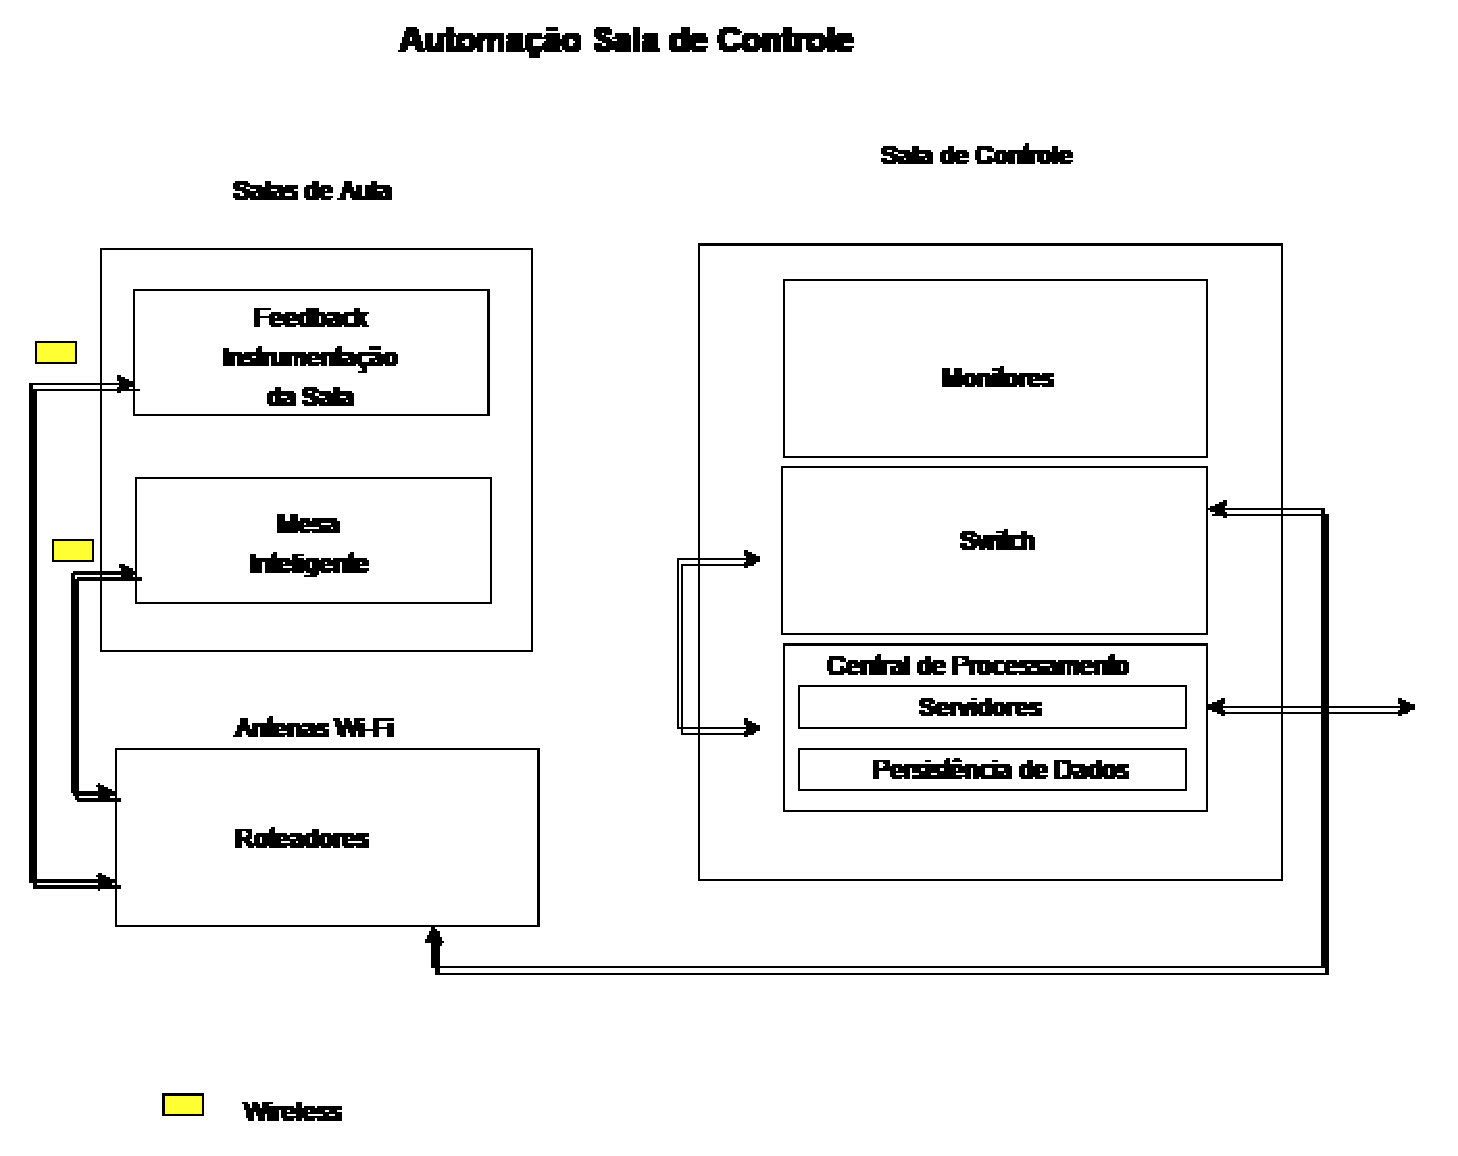
\includegraphics[keepaspectratio=true,scale=0.4]{figuras/automacao_sala_de_controle.eps}
  \caption{Sala de Controle}
  \label{fig:sala_cont}
\end{figure}

A conexão dos dispositivos com a sala de controle é representada nas figuras ~\ref{fig:plant_sup} e ~\ref{fig:plant_inf}.

\begin{figure}[!ht]
  \centering
  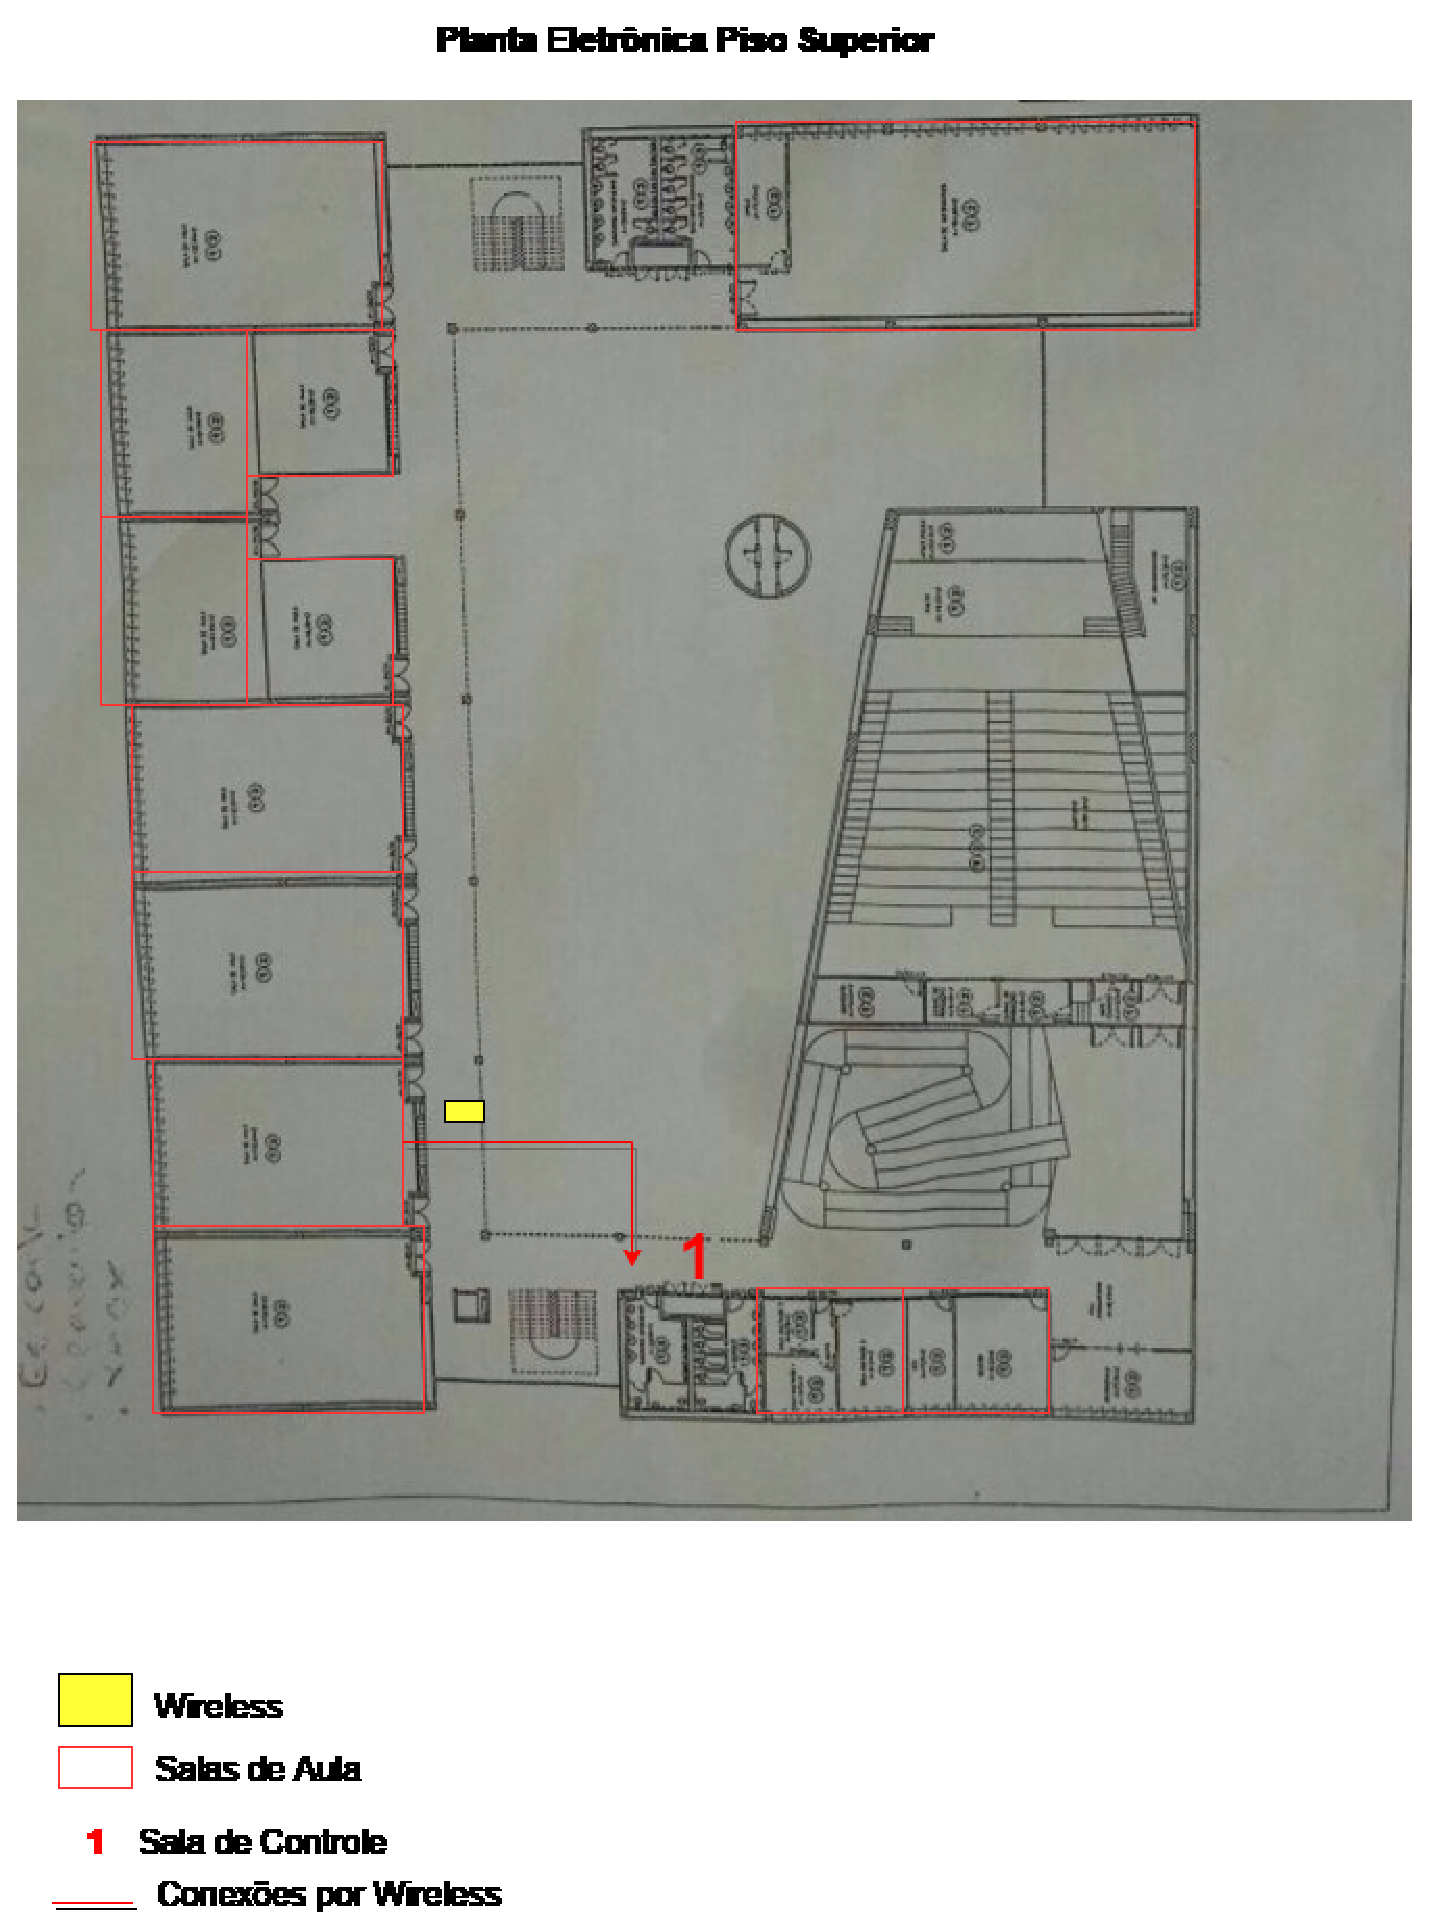
\includegraphics[keepaspectratio=true,scale=0.4]{figuras/planta_eletronica_superior.eps}
  \caption{Planta Eletrônica Piso Superior}
  \label{fig:plant_sup}
\end{figure}

\begin{figure}[!ht]
  \centering
  \includegraphics[keepaspectratio=true,scale=0.3]{figuras/planta_eletronica_inferior.eps}
  \caption{Planta Eletrônica Piso Inferior}
  \label{fig:plant_inf}
\end{figure}

Além de enviar e receber dados da sala de controle, alguns dispositivos se comunicam uns com os outros, como no caso das salas de aula, onde a mesa inteligente controla todos os dispositivos de automação presentes nas salas, funcionando como um painel de controle central pada cada uma delas, como é mostrado nas figuras ~\ref{fig:sala_aula} e ~\ref{fig:sala_comp}.

\begin{figure}[!ht]
  \centering
  \includegraphics[keepaspectratio=true,scale=0.3]{figuras/instrumentacao_da_sala.eps}
  \caption{Sala de Aula}
  \label{fig:sala_aula}
\end{figure}

\begin{figure}[!ht]
  \centering
  \includegraphics[keepaspectratio=true,scale=0.3]{figuras/automacao_sala_de_computadores.eps}
  \caption{Sala de Computadores}
  \label{fig:sala_comp}
\end{figure}











\chapter[Interfaces e Processamento de Software]{Interfaces e Processamento de Software}

\section{Estrutura do Banco de Dados}

O projeto do prédio inteligente/sustentável faz com que haja necessidade de armazenamento de dados. Os quais são gerados a partir da identificação diária do aluno em sala de aula, que é utilizado para o controle de acesso à cada aula, dos dados relacionados à produção e consumo de energia, que são gerenciados pelo Smart Grid e dados comuns.
Para o armazenamento de dados há algumas alternativas.
\begin{itemize}
  \item Servidores Locais
    \begin{itemize}
    \item Torre;
    \item Rack;
    \item Blade;
    \end{itemize}
  \item Dispositivos de Storage;
  \item Servidores e Nuvem;
\end{itemize}

Os servidores locais permitem com que dados possam ser acessados, alterados e adicionados por computadores ligados ao(s) servidor(es). Geralmente, são usados quando há uma grande transferência de dados entre as máquinas/servidores. Assim, podendo ser acessado com mais facilidade, agilidade, rapidez e segurança. Porém há um gasto maior com profissionais especializados em manutenção de tais servidores \cite{baguete}.
Os servidores do tipo Torre é o modelo mais básico, indicado para pequenas empresas, as quais não dispõem de uma sala de dados específica para armazenar os servidores. Tendo os seus componentes de hardware adaptados às necessidades e ao tamanho do projeto e/ou equipe \cite{anyconsulting}.
Os servidores do tipo Blade são formados por um microprocessador, barramentos e memória, e o conjunto de blades compartilha da mesma conexão de rede, refrigeração e fornecimento de energia. Seus componentes são armazenados dentro de um chassi ou gabinete. Mesmo tendo um tamanho reduzido, os servidores são úteis para o desenvolvimento de data centers e hospedagens de serviços web, pois, é mais flexível em relação à velocidade que a quantidade de armazenamento de dados vai crescendo, em vista que são modulares.
Os servidores racks atendem melhor grandes empresas que necessitam de uma infraestrutura de TI complexa. Possui um alto desempenho e tem um melhor aproveitamento do espaço, permitindo a retirada e inclusão de servidores de acordo com a demanda e necessidade de armazenamento \cite{anyconsulting}.
Os dispositivos de storage é uma solução confiável, além dos servidores locais, para o armazenamento de dados e arquivos. Porém, não tem capacidade para transferências frequentes dessas informações entre as máquinas que compõe o sistema. São apenas aparelhos que atuam como um HD (disco rígido), não possuindo uma interface, sistema operacional, que permita a transferência de dados, nem acesso múltiplo de computadores \cite{baguete}.
O gerenciamento de dados em servidores na Nuvem, é o armazenamento de dados online no servidor de empresas que forneçam esse serviço. Sendo uma alternativa mais em conta quando se trata do tamanho do empreendimento, quantidade de dados que serão armazenados e utilizados. Sendo online, o serviço fornecido depende muito mais da internet do contratante. O acesso às informações guardadas e à inserção/alteração dos dados, tem uma menor agilidade, rapidez e segurança quando se comparado à um servidor local. A segurança de um armazenamento em nuvem, depende mais da empresa à qual fornece o serviço. Então, os dados ficam vulneráveis aos ataques aos servidores da empresa \cite{baguete}.
A alternativa que mais se adequa a realidade do projeto, é o uso de um servidor local, assim, terá um acesso mais rápido aos dados, uma segurança maior e uma manutenibilidade de qualidade e rápida.
A Faculdade do Gama possui um servidor para atender suas necessidades, como o portal da FGA, sites de professores, dentre outros serviços. O servidor é do tipo Rack e está localizado na sala 36, do prédio UED. Portanto, os dados obtidos diariamente no projeto, serão armazenados no próprio servidor da faculdade, tendo em vista que ele está disponível para o nosso uso.
Para o banco de dados será estruturada uma arquitetura de processamento e armazenamento dos dados, utilizando o sistema de gerenciamento de dados MySQL (My Structured Query Language). O MySQL é um sistema de código aberto com base no sistema operacional Windows e muito utilizado por grandes empresas como a NASA(National Aeronautics and Space Administration), Banco Bradesco, entre outras. Esse sistema se destaca em relação aos outros quando o objetivo é obter velocidade de acesso aos dados armazenados, porém a base de dados sendo pequena não se nota diferença de comportamento em relação a velocidade de acesso entre o MySQL e outros sistemas. Utilizando o MySQL o responsável pela manutenção do sistema terá a sua disposição mais níveis de isolamento de transações que em outros sistemas como mostra a tabela ~\ref{table:niveis_isol}.

% Please add the following required packages to your document preamble:
% \usepackage{graphicx}
\begin{table}[]
\centering
\caption{Comparação Níveis de Isolamento.}
\label{table:niveis_isol}
\resizebox{\textwidth}{!}{%
\begin{tabular}{|l|c|c|c|}
\hline
Isolamento & \multicolumn{1}{l|}{Oracle} & \multicolumn{1}{l|}{SQL Server} & \multicolumn{1}{l|}{PostgreSQL} \\ \hline
Read uncommitted &  & x &  \\ \hline
Read committed & x & x & x \\ \hline
Repeatable read &  & x &  \\ \hline
Serializable & x & x & x \\ \hline
\end{tabular}%
}
\end{table}

Atualmente os sistemas de gerenciamento de banco de dados (SGBDs) suportam vários tipos de storage engines e até mais de uma no mesmo sistema. As engines dos SGBDs são responsáveis por criar, ler, atualizar,  e deletar (do inglês create, read, update and delete. CRUD) os dados no sistema e na tabela ~\ref{table:storage_engines} tem alguns exemplos de engines que são ou não transacionais e as engines que se integram perfeitamente ao sistema MySQL são InnoDB e MyISAM.

% Please add the following required packages to your document preamble:
% \usepackage{graphicx}
\begin{table}[]
\centering
\caption{Storage Engines}
\label{table:storage_engines}
\resizebox{\textwidth}{!}{%
\begin{tabular}{|c|c|c|}
\hline
Nome & Licença & Transacional \\ \hline
Aria & GPL & Não \\ \hline
BlitzDB & GPL & Não \\ \hline
Falcon & GPL & Sim \\ \hline
InnoDB & GPL & Sim \\ \hline
MyISAM & GPL & Não \\ \hline
InfiniDB & GPL & Não \\ \hline
TokuDB & GPL & Sim \\ \hline
WiredTiger & GPL & Sim \\ \hline
XtraDB & GPL & Sim \\ \hline
RocksDB & BSD & Sim \\ \hline
\end{tabular}%
}
\end{table}

O MyISAM é a engine nativa do MySQL e oferece um gerenciamento de dados mais conservativo deixando cada tabela em um arquivo diferente que pode ser comprimido com o comando myisamchk se for necessário diferentemente do InnoDB que armazena as tabelas em um espaço especial para as tabelas, o que impossibilita a otimização do espaço. Algumas funções são executadas com mais eficácia que no InnoDB por causa da complexidade do espaço especial das tabelas do InnoDB \cite{InnoDB}.
Em compatibilidade com o sistema de gerenciamento de banco de dados MySQL (Linguagem de Consulta Estruturada) o InnoDB se torna a opção mais viável para ser a engine do banco de dados. Além da compatibilidade com o MySQL o InnoDB difere de seu concorrente MyISAM por oferecer a função transacional que implica em um modo de funcionamento “tudo ou nada”. O sistema transacional preza a integridade dos dados, portanto se algum erro ocorrer ou faltar energia/conectividade o sistema não irá gravar os dados pela metade no banco de dados e executará um rollback para os dados anteriores ao erro. Enquanto o tempo de recuperação do MyISAM cresce de acordo com o tamanho do banco de dados a capacidade de rollback do InnoDB economiza tempo diante de uma falha \cite{InnoDB}.
Com base no estudo da equipe de Automação - Controle de Acesso, serão armazenados e renovados toda vez que o aluno utilizar a carteirinha um token. Além, de cada um possuir um chip, embutido em sua carteirinha. Armazenados então, um dado do tipo inteiro de 4 bytes\cite{microsoft1}, referente ao token. E inicialmente um array de char de 5 caracteres. Cada char possui um tamanho de 1 byte\cite{microsoft1}, tendo então, um dado referente ao chip da carteirinha de 5 bytes. Com isso temos que 5000 mil alunos utilizam 45000 bytes ou 4,5e-5 gigabytes.
Os dados que serão disponibilizados pelo trabalho da equipe responsável pelo Smart Grid, serão dois do tipo float, 4 bytes\cite{microsoft1} cada, e um do tipo date, 4 bytes\cite{microsoft1}. Respectivamente, um dado sobre o consumo diário, um outro da produção diária, e o dia referente ao consumo/produção, o que totaliza 20 bytes por dia ou 6e-7 gigabytes por mês.
Considerando cerca de 15 itens, entre sensores e outros dispositivos eletrônicos,  que geram dados por ambiente e 25 ambientes no prédio, o grupo de de automação - Instrumentação e Controle determinou que para cada dispositivo gerando 100 bytes por segundo, cerca de 0.3 gigabytes por mês com mais 5 gigabyte de aplicações para processamento de dados, sem mais dados armazenados de antemão totalizando 14 gigabytes por mês.
A quantidade de dados obtidos diariamente gerará na faixa de 14,0000006 gigabytes por mês além dos 5.0045 gigabytes já armazenados como dados fixos. Assim, serão armazenados no servidor Rack, já existente na faculdade, e gerenciados pelo InnoDB.

\section{Arquitetura do Aplicativo}

Como forma de informação para usuários do prédio e integração entre as mais diversas funcionalidades dele um aplicativo web-app servirá de ponte ligando os usuários as informações.
Um web-app é um site com domínio próprio que é acessado por meio de um navegador com o diferencial de ser responsivo, ou seja, sua funcionalidades são flexíveis de forma a permitir adaptação a qualquer dispositivo que o acesse.

\subsection{Model-View-Controller}

Para a arquitetura de software da aplicação web que será interligada ao uso do prédio, foram feitas diversas pesquisas e estudos, e a arquitetura escolhida foi a Model-View-Controller(MVC), em português modelo-visão-controlador.

MVC é um padrão de arquitetura de software que divide a representação da informação da interação do usuário com ele. Desta forma, alterações feitas na interface não afetam a manipulação de dados, e estes poderão ser reorganizados sem alterar a interface.

\begin{figure}[!ht]
  \centering
  \includegraphics[keepaspectratio=true,scale=0.45]{figuras/MVC.eps}
  \caption{Arquitetura Model-View-Controller}
  \label{fig:mvc}
\end{figure}

Model: É responsável pelo armazenamento dos dados, assim como a  validação e manipulação deles. A regra é simples: tudo que diz respeito à escrita, validação e leitura dos dados está dentro da camada model.
View: A camada de interação com o usuário e também de exibição de dados. Ela faz a  exibição dos dados, sendo ela por meio de um html ou xml.
Controller: É responsável por receber todas as requisições do usuário. Seus métodos, chamados actions, são responsáveis pela página, controlando qual model usar e qual view será mostrado ao usuário.
Neste projeto, tanto o back-end quanto o front-end farão uso do framework Rails. Sua organização de pastas segue a organização descrita na figura ~\ref{fig:pastas}:

\begin{figure}[!ht]
  \centering
  \includegraphics[keepaspectratio=true,scale=0.4]{figuras/pastas.eps}
  \caption{Estrutura de Diretórios do Aplicativo}
  \label{fig:pastas}
\end{figure}

\subsection{Model-View-ViewModel}

MVVM é um padrão arquitetural, que impõe uma separação da interface do usuário XAML (a View) dos dados subjacentes (a Model) através de uma classe que serve como um intermediário entre a View e a Model (ViewModel). View e ViewModel geralmente são conectadas através de ligações de dados (binding) definidas no arquivo XAML.
A Model é responsável por realizar o gerenciamento e validação de dados bem como o estado da aplicação.
A View é a interface de usuário, exibe informações ao usuário, e responde às interações.
A ViewModel é a classe que estabelece a conexão entre View e Model, atualizando os dados na Model, que foram modificados através dos eventos na View.
Os testes são realizados sobre a ViewModel, pois é ela que possui toda a lógica necessária para que a View possa funcionar de forma esperada, e a ViewModel não tem conhecimento sobre nada na View.

\begin{figure}[!ht]
  \centering
  \includegraphics[keepaspectratio=true,scale=0.6]{figuras/MVVM.eps}
  \caption{Arquitetura MVVM}
  \label{fig:mvvm}
\end{figure}

\section{Escolha da Arquitetura}

Considerando os padrões MVVM (Model-View-ViewModel) e MVC (Model-View-Controller), não existe um superior ao outro, mas sim qual se adequa melhor ao projeto a ser desenvolvido. No caso do Prédio Sustentável, a aplicação web será construída utilizando Ruby on Rails, que por padrão é MVC.

\section{Protótipo de Alta Fidelidade}
\label{sec:prot}
Para melhor entendimento do aplicativo foi realizado um protótipo de alta fidelidade onde é possível vizualizar uma representação do aplicativo, suas funcionalidades e a forma de acesso a elas.

Um protótipo de alta fidelidade é um artefato que se assemelha ao produto final apoiando a avaliação de todos os detalhes de um design de forma a trazer mais clareza para desenvolvedores e usuários.

O protótipo de alta fidelidade do aplicativo foi estabelecido de acordo com as imagens que estão disponíveis no anexo \ref{protot}.

\begin{figure}[!ht]
  \centering
  \includegraphics[keepaspectratio=true,scale=0.6]{figuras/prot-0.eps}
  \caption{Protótipo do Login do Aplicativo}
\end{figure}
